\RequirePackage{luatex85}
\documentclass[eqno]{ltjsarticle}
\usepackage{luatexja-fontspec}
\usepackage[a4paper, top=25mm, bottom=25mm, left=25mm, right=25mm]{geometry}
\usepackage{luatexja} 
\usepackage{multicol,amsmath,amssymb,mathtools,ascmac,amsthm,amscd,physics,comment,dcolumn,titlesec,mathrsfs,test,tikz-cd,enumitem}
\usetikzlibrary{arrows.meta,calc}
\titleformat*{\section}{\Large\bfseries}
\setlength{\parindent}{0pt}
\usepackage[most]{tcolorbox}
\tikzset{every picture/.style={remember picture,baseline=(current bounding box.center)}}
\usetikzlibrary{decorations.pathmorphing}
%\everymath{\displaystyle}
\begin{document}
\title{三角圏上のBridgeland安定性条件}
\date{}
\author{大阪大学大学院理学研究科数学専攻\\山本 雄大}
\maketitle
\tableofcontents
\section{三角圏の定義}
\begin{defn}\cite[p.170]{KS06}
	以下の条件をみたす圏$\C$を前加法圏(preadditive category)という.
	\vspace{-3mm}
	\begin{itemize}
		\item[(i)]
			任意の$X,Y\in\C$に対して,射の集合$\Hom_{\C}(X,Y)$が加法群になる.
		\item[(ii)]
			任意の$X,Y,Z\in\C$に対して,合成写像
		\[
			\begin{array}{ccccc}
				\circ\colon\Hom_{\C}(Y,Z) \times \Hom_{\C}(X,Y) & \longrightarrow & \Hom_{\C}(X,Z) \\
				\rotatebox{90}{\in}& &\rotatebox{90}{\in}\\
				(g, f) & \longmapsto & g \circ f& .
					\end{array}
\]
が双線型である.つまり,任意の$g,g'\in\Hom_{\C}(Y,Z),\ f,f'\in\Hom_{\C}(X,Y)$に対して,
\begin{gather*}
	(g+g')\circ f = g\circ f + g'\circ f\\
	g\circ(f+f') = g\circ f + g\circ f'.
\end{gather*}
が成り立つ.
	\end{itemize}
\end{defn}

\begin{defn}\cite[p.171]{KS06}
	$\C$を前加法圏とする.このとき,対象$X\oplus Y\in\C$と$\iota_{X}\in\Hom_{\C}(X,X\oplus Y),\iota_{Y}\in\Hom_{\C}(Y,X\oplus Y)$の三つ組$(X\oplus Y,\iota_X,\iota_Y)$であって,以下の普遍性を満たすものを$X,Y\in\C$の直和(direct sum)という.
	\[\begin{tikzcd}
		X\ar[r,"\iota_X"]\ar[rd,"f_X",swap]& X\oplus Y\ar[d,dotted,"\exists !h",swap] &Y\ar[l,"\iota_Y",swap]\ar[ld,"f_Y"]\\
																			 &Z&.
\end{tikzcd}\]
任意の$Z\in\C$と$f_X\in\Hom_{\C}(X,Z),\ f_Y\in\Hom_{\C}(Y,Z)$に対して,$h\circ \iota_X=f_X,\ h\circ\iota_Y=f_Y$となる$h\in\Hom_{\C}(X\oplus Y,Z)$が一意に存在する.
\end{defn}

\begin{defn}\cite[p.171]{KS06}
	以下の条件をみたす前加法圏$\C$を加法圏(additive category)という.
	\vspace{-3mm}
	\begin{itemize}
	\item[(i)]零対象(始対象かつ終対象)である$0\in\C$をを持つ.
	\item[(ii)]任意の対象$X,Y\in\C$に対し直和$X\oplus Y$が存在する.
	\end{itemize}
	\vspace{-3mm}
\end{defn}

\begin{defn}\cite[p.171]{KS06}
	 	加法圏$\C,\D$に対し,函手$F\colon\C\to\D$が以下の条件を満たすとき加法函手(additve functor)という.
		\begin{itemize}
			\item[(1)]
				任意の$X,Y\in\C$に対し,
				\[
			\begin{array}{ccccc}
				F\colon\Hom_{\C}(X,Y) & \longrightarrow & \Hom_{\D}(F(X),F(Y)) \\
				\rotatebox{90}{\in}& &\rotatebox{90}{\in}\\
				f & \longmapsto & F(f)&.
					\end{array}
				\]
				が加法群の準同型写像になっている.つまり任意の$f,g \in\Hom_{\C}(X,Y)$に対し,
				\[F(f + g) = F(f) + F(g).\]
				となる.
			\item[(2)]
				$0\in\C$に対し,$F(0)=0$
			\item[(3)]
			直和を保つ.つまり,任意の対象$X,Y\in\C$に対して以下が成り立つ.
				\[F(X\oplus Y)\simeq F(X)\oplus F(Y).\]
		\end{itemize}
\end{defn}

\begin{defn}\cite[p.175]{KS06}
	$\C$を加法圏とする.このとき,$f\in\Hom_{\C}(X,Y)$の核(kernel)とは$\Ker f\in\C$と$\ker f\in\Hom_{\C}(\Ker f,X)$の組$(\Ker f,\ker f)$であって,以下の普遍性をみたすものである.
	\[\begin{tikzcd}
		K\ar[rd,"k"]\ar[d,"\exists !h",dotted,swap]\\
		\Ker f\ar[r,"\ker f",swap]&X\ar[r,"f",swap]&Y.
\end{tikzcd}\]
\begin{itemize}
	\item[(i)]
		$f\circ\ker f=0$
	\item[(ii)]
		任意の$K\in\C$と$k\in\Hom_{\C}(K,X)$で$f\circ k=0$を満たすものに対して,一意に$h\in\Hom_{\C}(K,\Ker f)$が存在して,$\ker f\circ h=k$となる.
\end{itemize}
$f\in\Hom_{\C}(X,Y)$の$\C$の反対圏での核を余核(cokernel)とよび,$(\Cok f,\cok f)$と記す.\\
また,$f$の像(Image) $\Im f$,余像(coimage) $\Coim f$を以下のように定義する.
\[\Im f\coloneq \Ker(\cok f)\quad \Coim f\coloneq \Cok(\ker f).\]
このとき,普遍性により以下の図式を可換にする射$\Coim f\to \Im f$が一意的に存在することがわかる.
	\[\begin{tikzcd}
		\Ker f\ar[r,"\ker f"]& X \ar[r,"f"]\ar[d,"p",swap]& Y\ar[r, "\cok f"]& \Cok f\\
												 &\Coim f\ar[ru,dotted]\ar[r,dotted] & \Im f\ar[u,"i",swap].
\end{tikzcd}\]
ただし,$p=\ker(\cok f),\, i=\cok(\ker f)$とした.
\end{defn}

\begin{defn}\cite[p.175]{KS06}
	加法圏$\A$が以下を満たすとき,アーベル圏(abelian category)という:
	\vspace{-3mm}
	\begin{itemize}
		\item[(i)]
			$\A$の任意の射$f$に対し,核$\Ker f$と余核$\Cok f$が存在する.
		\item[(ii)]
			$\A$の任意の射$f$に対し,自然な準同型\ $\Coim(f)\simeq\Im f$が同型となる.
	\end{itemize}
\end{defn}
	加法圏$\D$と自己同値函手$[1]\colon\D\to\D$与えられているとき,$\D$における三角形とは以下の形の射の列をいう.
	\[X\xrightarrow{f}Y\xrightarrow{g} Z\xrightarrow{h} X[1].\]

	\begin{defn}\cite[p.243]{KS06}
	加法圏$\D$に自己同値函手$[1]$と完全三角形(distinguished triangle)と呼ばれる三角形の集合が与えられていて,これらが以下の条件を満たすとき,$\D$を三角圏(triangulated category)と呼ぶ.三角形が完全三角形であるとき,「三角形が完全である.」とも表現し,以下の記述も用いることにする.
	\[X\xrightarrow{f}Y\xrightarrow{g} Z\xrightarrow{h} X[1]\hspace{3mm}(完全). \]
	\vspace{-3mm}
	\begin{itemize}
		\item[(TR1)]
			任意の$X\in\D$に対して,
			\[X\xrightarrow{\id_X}X\rightarrow 0 \rightarrow X[1].\]
			は完全三角形である.
		\item[(TR2)]
		以下の2つの三角形とその間の射$f,g,h$が
			\[
		\begin{tikzcd}
			X_1\ar[r]\ar[d,"f"]& X_2\ar[r]\ar[d,"g"]& X_3\ar[r]\ar[d,"h"] & X_1[1]\ar[d,"f\texttt{[1]}"]\\
			Y_1\ar[r]& Y_2\ar[r]& Y_3\ar[r] & Y_1[1].\\
		\end{tikzcd}
			\]
		このとき,$f,g,h$が同型で$X_1\rightarrow X_2\rightarrow X_3 \rightarrow X_1[1]$が完全三角形なら$Y_1\rightarrow Y_2\rightarrow Y_3 \rightarrow Y_1[1]$も完全三角形である.
		\item[(TR3)]
			任意の射$X\xrightarrow{f}Y$は,$X\xrightarrow{f} Y\rightarrow Z \rightarrow X[1]$と完全三角形に拡張できる.
	\item[(TR4)]
		三角形
		\[X_1\xrightarrow{u} X_2\xrightarrow{v} X_3\xrightarrow{w}  X_1[1].\]
		が完全三角形であることと
		\[X_2\xrightarrow{v} X_3\xrightarrow{w} X_1[1]\xrightarrow{-u[1]}  X_2[1].\]
		が完全三角形であることが同値である.

	\item[(TR5)]
以下の2つの完全三角形と図式を可換にする$f,g$が存在したとする.
		\[
		\begin{tikzcd}
			X_1\ar[r]\ar[d,"f"]& X_2\ar[r]\ar[d,"g"]& X_3\ar[r]\ar[d,"h",dotted] & X_1[1]\ar[d,"f\texttt{[1]}"]\\
			Y_1\ar[r]& Y_2\ar[r]& Y_3\ar[r] & Y_1[1].\\
		\end{tikzcd}
	\]
	このとき,すべての四角形を可換にする$h$が存在する.

	\item[(TR6)]
		(八面体公理)3つの完全三角形
			\[
				\begin{tikzcd}[row sep=5pt]
			X \ar[r,"f"]& Y\ar[r,"h"]& Z' \ar[r]& X[1]\\
			X \ar[r,"g\circ f"]& Z\ar[r,"l"]& Y' \ar[r]& X[1]\\
			Y \ar[r,"g"]& Z\ar[r,"k"]& X' \ar[r]& Y[1].\\
		\end{tikzcd}
			\]
			に対して,以下の図式のすべての四角形を可換にし,4行目を完全三角形にするような$u\in\Hom_{\D}(Z',Y'),v\in\Hom_{\D}(Y',X'),w\in\Hom_{\D}(X',Z'[1])$が存在する.
			\[
		\begin{tikzcd}
			X \ar[r,"f"]\ar[d,equal]& Y\ar[r,"h"]\ar[d,"g",swap]& Z'\ar[d,"u",dotted] \ar[r]& X[1]\ar[d,equal]\\
			X \ar[r,"g\circ f"]\ar[d,"f",swap]& Z\ar[r,"l"]\ar[d,equal]& Y'\ar[d,"v",dotted] \ar[r]& X[1]\ar[d,"f\texttt{[1]}"]\\
			Y \ar[r,"g"]\ar[d,"h",swap]& Z\ar[r,"k"]\ar[d,"l",swap]& X' \ar[r]\ar[d,equal]& Y[1]\ar[d,"h\texttt{[1]}"]\\
			Z' \ar[r,"u",dotted]& Y'\ar[r,"v",dotted]& X' \ar[r,"w",dotted]& Z'[1].\\
		\end{tikzcd}
			\]
	\end{itemize}
\end{defn}

\begin{defn}\cite[p.243]{KS06}
三角圏 $\D$ において,2つの完全三角形
\[
X \xrightarrow{f} Y \xrightarrow{g} Z \xrightarrow{h} X[1], \quad
X' \xrightarrow{f'} Y' \xrightarrow{g'} Z' \xrightarrow{h'} X'[1].
\]
が与えられているとする.

このとき,射の三つ組 $(\alpha, \beta, \gamma)$(ただし $\alpha \colon X \to X'$,$\beta \colon Y \to Y'$,$\gamma \colon Z \to Z'$)が以下の図式が可換にするとき,完全三角形の間の射(morphism of triangles)であるという:
\[
\begin{tikzcd}
X \arrow{r}{f} \arrow{d}{\alpha} & Y \arrow{r}{g} \arrow{d}{\beta} & Z \arrow{r}{h} \arrow{d}{\gamma} & X[1] \arrow{d}{\alpha[1]} \\
X' \arrow{r}{f'} & Y' \arrow{r}{g'} & Z' \arrow{r}{h'} & X'[1].
\end{tikzcd}
\]
すなわち,以下が成り立つ:
\[
\beta \circ f = f' \circ \alpha, \quad
\gamma \circ g = g' \circ \beta, \quad
\alpha[1] \circ h = h' \circ \gamma.
\]
\end{defn}

\section{三角圏の基本的な性質}
\begin{prop}\cite[p.245]{KS06}\label{gf=0}
三角圏 $\D$ において,完全三角形
\[
X \xrightarrow{f} Y \xrightarrow{g} Z \xrightarrow{h} X[1].
\]
が与えられたとき,合成 $g \circ f = 0$ が成り立つ.
\end{prop}

\begin{proof}
三角圏の公理 (TR1) と(TR5)により,以下の図式
		\[
\begin{tikzcd}
	X\ar[r,"\id"]\ar[d,"\id"]&X \ar[r]\ar[d,"f"]& 0\ar[r]\ar[d]& X[1]\ar[d,"f\texttt{[1]}"]\\
	X\ar[r,"f"]&Y \ar[r,"g"]& Z\ar[r]& X[1].
\end{tikzcd}
	\]
	が可換になることから$g\circ f = 0$である.
\end{proof}

\begin{prop}\cite[p.245]{KS06}
三角圏 $\D$ において,対象 $X \in \D$ と同型射 $f \colon X \xrightarrow{\sim} Y$ が与えられたとする.
このとき,三角
\[
X \xrightarrow{f} Y \to 0 \to X[1].
\]
は完全三角形である.
\end{prop}

\begin{proof}
三角圏の公理 \textnormal{(TR1)} により,任意の対象 $X$ に対して恒等射による完全三角形と以下の完全三角形の同型
		\[
\begin{tikzcd}
	X\ar[r,"f"]\ar[d,equal]&Y \ar[r]\ar[d,"f\inv"]& 0\ar[r]\ar[d]& X[1]\ar[d,equal]\\
	X\ar[r,"\id"]&X \ar[r,"g"]& 0\ar[r]& X[1].
\end{tikzcd}
	\]
	が存在するので,上の行が完全三角形であることがわかる.
\end{proof}

\begin{defn}\cite[p.245]{KS06}
	三角圏$\D$からアーベル圏$\A$への加法函手$H\colon \D\to\A$が,$\D$における任意の完全三角形:
	\[X\xrightarrow{f}Y\xrightarrow{g}Z\xrightarrow{h}X[1].\]
	に対して,$\A$において
	\[H(X)\xrightarrow{H(f)}H(Y)\xrightarrow{H(g)}H(Z).\]
	が完全列になるとき,コホモロジー的であるという.
\end{defn}

\begin{prop}\cite[p.245]{KS06}
	$\D$を三角圏,$W\in \D$としたとき,函手
	\begin{gather*}
		\Hom_{\D}(W,-)\colon \D\to\Mod\ZZ \\
		\Hom_{\D}(-,W)\colon \D^{\mathrm{op}}\to\Mod\ZZ\ .
	\end{gather*}
	はコホモロジー的函手である.
\end{prop}
\begin{proof}
	$X\rightarrow Y \rightarrow Z\rightarrow X[1]$を完全三角形,$W\in\D$とする.このとき,以下の完全列
	\[\Hom_{\D}(W,X)\xrightarrow{\Hom_{\D}(W,f)}\Hom_{\D}(W,Y)\xrightarrow{\Hom_{\D}(W,g)}\Hom_{\D}(W,Z).\]
	が完全であることを示す.命題\ref{gf=0}より,$\Im(\Hom_{\D}(W,f))\subset \Ker(\Hom_{\D}(W,g))$がわかる.
	逆の包含に関してはTR4,TR5より,$g\circ\varphi = 0$をみたす$\varphi\colon W\to Y$を任意にとると,以下の図式を可換にする$\psi\colon W\to X$が存在する.
		\[
\begin{tikzcd}
	W\ar[r,"\id"]\ar[d,dotted,"\psi"]&W \ar[r]\ar[d,"\varphi"]& 0\ar[r]\ar[d]& W[1]\ar[d,"\psi\texttt{[1]}"]\\
	X\ar[r,"f"]&Y \ar[r,"g"]& Z\ar[r]& X[1].
\end{tikzcd}
	\]
つまり,$\varphi = f\circ\psi$である.したがって,$\Im(\Hom_{\D}(W,f))= \Ker(\Hom_{\D}(W,g))$が示された.
\end{proof}



\begin{prop}\cite[p.246]{KS06}
三角圏 $\D$ において,次の2つの完全三角形
\[
X \xrightarrow{f} Y \xrightarrow{g} Z \xrightarrow{h} X[1], \quad
X' \xrightarrow{f'} Y' \xrightarrow{g'} Z' \xrightarrow{h'} X'[1].
\]
とその間の射,
\[
\begin{tikzcd}
X \arrow{r}{f} \arrow{d}{\alpha}[swap]{\sim} & Y \arrow{r}{g} \arrow{d}{\beta}[swap]{\sim} & Z \arrow{r}{h} \arrow[dotted]{d}{\gamma} & X[1] \arrow{d}{\alpha[1]} \\
X' \arrow{r}{f'} & Y' \arrow{r}{g'} & Z' \arrow{r}{h'} & X'[1].
\end{tikzcd}
\]
が与えられており,$\alpha, \beta$ が同型であれば,$\gamma$ も同型となる.
\end{prop}
\begin{proof}
	$W\in\D$を任意にとり,$\Hom_{\D}(W,-)$を作用させるとコホモロジー的函手であることにより,以下の完全列が存在する.
\[\begin{tikzcd}
	\Hom_{\D}(W,X)\ar[r]\ar[d,"\rotatebox{90}{\sim}"]&\Hom_{\D}(W,Y)\ar[r]\ar[d,"\rotatebox{90}{\sim}"]&\Hom_{\D}(W,Z)\ar[r]\ar[d]&\Hom_{\D}(W,X[1])\ar[r]\ar[d,"\rotatebox{90}{\sim}"]&\Hom_{\D}(W,Y[1])\ar[d,"\rotatebox{90}{\sim}"]\\
	\Hom_{\D}(W,X')\ar[r]&\Hom_{\D}(W,Y')\ar[r]&\Hom_{\D}(W,Z')\ar[r]&\Hom_{\D}(W,X'[1])\ar[r]&\Hom_{\D}(W,Y'[1]).
\end{tikzcd}\]	
5項補題により,$\Hom_{\D}(W,\gamma)$が同型である.$W\in\D$は任意なので,米田の補題より$\gamma$は同型である.
\end{proof}

\begin{cor}\cite[p.246]{KS06}
三角圏 $\D$ において,射 $f \colon X \to Y$ に対して,
2つの完全三角形
\[
X \xrightarrow{f} Y \xrightarrow{g} Z \xrightarrow{h} X[1], \quad
X \xrightarrow{f} Y \xrightarrow{g'} Z' \xrightarrow{h'} X[1].
\]
が存在するとする.このとき,対象 $Z, Z'$ は同型であり,さらに完全三角形の間の同型射
\[
\begin{tikzcd}
X \arrow{r}{f} \arrow[equal]{d} & Y \arrow{r}{g} \arrow[equal]{d} & Z \arrow{r}{h} \arrow[dashed]{d}{\varphi} & X[1] \arrow[equal]{d} \\
X \arrow{r}{f} & Y \arrow{r}{g'} & Z' \arrow{r}{h'} & X[1].
\end{tikzcd}
\]
が存在する.このような$Z$を同型類から$1$つ選び,$f$の写像錘(mapping cone)と呼び,記号$\Cone(f)$と記す.
\end{cor}

\begin{cor}
三角圏 $\D$ における完全三角形
\[
X \xrightarrow{f} Y \xrightarrow{g} Z \xrightarrow{h} X[1].
\]
に対して,以下が成り立つ:

\begin{enumerate}
  \item $g$ が全射であることと$h = 0$であることは同値である.
  \item $g$ が単射であることと$f = 0$であることは同値である.
  \item $h = 0$ ならば,$Y \cong X \oplus Z$ が成り立ち,この三角は
  \[
  X \xrightarrow{\iota} X \oplus Z \xrightarrow{\pi} Z \xrightarrow{0} X[1].
  \]
  に同型である(ただし $\iota$ は自然な包含、$\pi$ は射影).
\end{enumerate}
\end{cor}
\begin{proof}
	命題\ref{gf=0}より,$h\circ g = 0$であり,$g$が全射なら$h=0$.逆に,任意の$W\in\D$に対して,
\[
	\Hom_{\D}(X[1],W)\xrightarrow{\Hom_{\D}(h,W)}\Hom_{\D}(Z,W)\xrightarrow{\Hom_{\D}(g,W)}\Hom_{\D}(Y,W).
\]	
が完全列なので,$h=0$なら,$\Hom_{\D}(g,W)$は単射である.したがって$g$は全射である.2は双対的に示される.\\
3について,$h=0$とすると,
\begin{gather*}
	0\rightarrow\Hom_{\D}(Z,W)\rightarrow\Hom_{\D}(Y,W)\rightarrow\Hom_{\D}(X,W)\rightarrow 0,\\
	0\rightarrow\Hom_{\D}(W,X)\rightarrow\Hom_{\D}(W,Y)\rightarrow\Hom_{\D}(W,Z)\rightarrow 0.
\end{gather*}
が短完全列になり,とくに$W=X,Z$として,$f'\circ f =\id_X,\ g\circ g'=\id_Z$なる$f',g'$の存在がわかり,短完全列
\[
0\rightarrow X \xrightarrow{f} Y \xrightarrow{g} Z\rightarrow 0 .
\]
が分裂して$Y\simeq X\oplus Z$となる.
\end{proof}

\begin{prop}\cite[p.247]{KS06}
三角圏 $\D$ において,次の2つの完全三角形
\[
X \rightarrow Y \rightarrow Z \rightarrow X[1], \quad
X' \rightarrow Y' \rightarrow Z' \rightarrow X'[1].
\]
が与えられているとする.

また,射$g\colon Y\to Y'$ が与えられており,さらに
\[
\Hom_{\D}(X, Z') = \Hom_{\D}(X, Z'[-1]) = 0.
\]
が成り立つとする.このとき,ある一意な射$f\colon X\to X'\quad h\colon Z\to Z'$が存在して,以下の図式が可換になる:
\[
\begin{tikzcd}
	X \arrow{r} \arrow[dotted]{d}{\exists !f} & Y \arrow{r} \arrow{d}{ g} & Z \arrow{r} \arrow[dotted]{d}{\exists !h} & X[1] \arrow[dotted]{d}{f[1]} \\
X' \arrow{r} & Y' \arrow{r} & Z' \arrow{r} & X'[1].
\end{tikzcd}
\]
すなわち,$(f,g,h)$ は完全三角形の間の射をなす.
\end{prop}
\begin{proof}
	コホモロジー的函手$\Hom_{\D}(X,-)$を2行目に作用させると,
	\[0=\Hom_{\D}(X,Z'[-1])\rightarrow \Hom_{\D}(X,X') \rightarrow \Hom_{\D}(X,Y') \rightarrow \Hom_{\D}(X,Z')=0.\]
	という完全列が得られ,可換にする一意的な射$f$の存在がわかる.同様に,$\Hom_{\D}(-,Z')$を1行目に作用させて,$\Hom_{\D}(X[1],Z')\simeq \Hom_{\D}(X,Z'[-1])$を用いれば,一意的な射$h$の存在もわかる.

\end{proof}

\section{アーベル圏の導来圏の定義}

\begin{defn}\cite[p.300]{KS06}
$\A$ をアーベル圏とする.このとき,$\A$ における複体の圏 $\mathsf{C}(\A)$ を次のように定める:

対象$X^\bullet\in\Ob(C(\A))$は,$\ZZ$-次付き加群の族 $\{X^n\}_{n \in \ZZ}$ と,各 $n \in \ZZ$ に対する射 $d_{X}^n: X^n \to X^{n+1}$ の組
  \[
		X^\bullet = ( \quad \cdots \xrightarrow{d_{X}^{n-2}} X^{n-1} \xrightarrow{d_{X}^{n-1}} X^n \xrightarrow{d_{X}^n} X^{n+1} \xrightarrow{d_{X}^{n+2}} \cdots \quad ).
  \]
	であって,すべての $n \in \mathbb{Z}$ に対して $d_{X}^{n+1} \circ d_{X}^n = 0$ を満たすものとする.

	$X^\bullet , Y^\bullet\in\Ob(\mathsf{C}(\A))$に対し,射$f^\bullet\in \Hom_{\mathsf{C}(\A)}(X^\bullet,Y^\bullet)$ は,各次数 $n \in \mathbb{Z}$ における射 $f^n: X^n \to Y^n$ の族
  \[
    f^\bullet = \{f^n\}_{n \in \mathbb{Z}}.
  \]
  であって,任意の $n \in \mathbb{Z}$ に対して
  \[
    d_Y^n \circ f^n = f^{n+1} \circ d_X^n.
  \]
  を満たすものとする.すなわち,以下の図式におけるすべての四角形を可換にするものである.
		\[
\begin{tikzcd}[column sep=large, row sep=large]
  \cdots \ar[r] &
  X^{n-1} \ar[r,"d_X^{n-1}"] \ar[d,"f^{n-1}"'] &
  X^n \ar[r,"d_X^n"] \ar[d,"f^n"'] &
  X^{n+1} \ar[r,"d_X^{n+1}"] \ar[d,"f^{n+1}"'] &
  \cdots \\
  \cdots \ar[r] &
  Y^{n-1} \ar[r,"d_Y^{n-1}"] &
  Y^n \ar[r,"d_Y^n"] &
  Y^{n+1} \ar[r,"d_Y^{n+1}"] &
	\cdots .
\end{tikzcd}
	\]
\end{defn}

\begin{defn}\cite[p.272]{KS06}
	$\mathcal{A}$ をアーベル圏とし,$X^\bullet, Y^\bullet \in \mathsf{C}(\mathcal{A})$ を複体とする.2つの複体の射 $f^\bullet, g^\bullet: X^\bullet \to Y^\bullet$ が次の条件をみたすとき,$f^\bullet$と$g^\bullet$はホモトピック(homotopic)であるという:\\
	$\mathcal{A}$ における射の族 $\{h^n: X^n \to Y^{n-1}\}_{n \in \mathbb{Z}}$ が存在して,任意の $n \in \mathbb{Z}$ に対して
\[
  f^n - g^n = d_Y^{n-1} \circ h^n + h^{n+1} \circ d_X^n.
\]
を満たす.このような射の族 $h^\bullet = \{h^n\}_{n \in \mathbb{Z}}$ をホモトピーと呼ぶ.このとき,$f^\bullet \overset{\mathrm{h.e.}}{\sim} g^\bullet$ と記す.
\[\begin{tikzcd}[column sep=large, row sep=large]
  \cdots \ar[r] &
	X^{n-1} \ar[r,"d_X^{n-1}"] \ar[d,"f^{n-1}"',"g^{n-1}"] \ar[dl,dotted,"h^{n-1}"description] &
  X^n \ar[r,"d_X^n"] \ar[d,"f^n"',"g^n"] \ar[dl,dotted,"h^n"description] &
	X^{n+1} \ar[r,"d_X^{n+1}"] \ar[d,"f^{n+1}"',"g^{n+1}"] \ar[dl,dotted,"h^{n+1}"description] &
	\cdots\ar[dl,dotted,"h^{n+2}"description] \\
  \cdots \ar[r] &
  Y^{n-2} \ar[r,"d_Y^{n-2}"'] &
  Y^{n-1} \ar[r,"d_Y^{n-1}"'] &
  Y^n \ar[r,"d_Y^n"'] &
  \cdots .
\end{tikzcd}
\]

\end{defn}

\begin{lemm}\cite[p.300]{KS06}\label{lem:well_defined_composition}
$\mathsf{C}(\A)$ におけるホモトピー関係 $\overset{\mathrm{h.e.}}{\sim}$ は,射の集合上の同値関係であり,さらに射の合成と整合している.すなわち,以下が成り立つ:
\begin{enumerate}
  \item 任意の複体の射 $f^\bullet: X^\bullet \to Y^\bullet$ に対して $f^\bullet \overset{\mathrm{h.e.}}{\sim} f^\bullet$.
  \item $f^\bullet \overset{\mathrm{h.e.}}{\sim} g^\bullet$ ならば $g^\bullet \overset{\mathrm{h.e.}}{\sim} f^\bullet$.
  \item $f^\bullet \overset{\mathrm{h.e.}}{\sim} g^\bullet$ および $g^\bullet \overset{\mathrm{h.e.}}{\sim} k^\bullet$ ならば $f^\bullet \overset{\mathrm{h.e.}}{\sim} k^\bullet$.
  \item 複体 $X^\bullet, Y^\bullet, Z^\bullet$ に対し,$f^\bullet, g^\bullet: X^\bullet \to Y^\bullet$ が $f^\bullet \overset{\mathrm{h.e.}}{\sim} g^\bullet$ かつ $u^\bullet: Y^\bullet \to Z^\bullet$ が任意の複体の射とすると,$u^\bullet \circ f^\bullet \overset{\mathrm{h.e.}}{\sim} u^\bullet \circ g^\bullet$.
  \item 同様に,$v^\bullet: W^\bullet \to X^\bullet$ を任意の複体の射とすると,$f^\bullet \circ v^\bullet \overset{\mathrm{h.e.}}{\sim} g^\bullet \circ v^\bullet$.
\end{enumerate}
\end{lemm}

\begin{proof}
	1.\ 任意の$f\in\Mor(\mathsf{C}(\A)))$に対して,$f^n -f^n  = 0 = d^{n-1}\circ 0 + 0\circ d^n$なので,$f\overset{\mathrm{h.e.}}{\sim}f$.\\
	2.\ $f \overset{\mathrm{h.e.}}{\sim}g$のとき,$f^n -g^n  = d^{n-1}\circ h^{n} + h^{n+1}\circ d^n$となる$\{h^n\}_{n\in\ZZ}$が存在するが,$g^n -f^n  = d^{n-1}\circ (-h^{n}) + (-h^{n+1})\circ d^n$なので,$g \overset{\mathrm{h.e.}}{\sim}f$\\
	3.\ $f^n -g^n  = d^{n-1}\circ h^{n} + h^{n+1}\circ d^n$かつ,$g^n -k^n  = d^{n-1}\circ h'^{n} + h'^{n+1}\circ d^n$なので,$f^n - k^n =d^{n-1}\circ (h^{n} + h'^n ) + (h^{n+1} + h'^{n+1})\circ d^n $\\
	4.\ $f^n -g^n  = d^{n-1}\circ h^{n} + h^{n+1}\circ d^n$を用いて,$u^n\circ f^n -u^n\circ g^n  = u^n\circ d^{n-1}\circ h^{n} + u^n\circ h^{n+1}\circ d^n = d^{n-1}\circ (u^{n-1}\circ h^n) + (u^n\circ h^{n+1})\circ d^n$となる.したがって,ホモトピー$\{u^n\circ h^{n+1}\}_{n\in\ZZ} $が構成できた.5.も同様に構成できる.
\end{proof}

\begin{defn}\cite[p.273]{KS06}
$\A$ をアーベル圏とする.補題~\ref{lem:well_defined_composition} により,ホモトピー関係 $\overset{\mathrm{h.e.}}{\sim}$ は $\mathsf{C}(\A)$ の射の集合上の同値関係を定め,かつ合成と整合している.

このとき,以下のようにして $\A$ 上のホモトピー圏 $\mathsf{K}(\A)$ を定義する:

\begin{itemize}
  \item 対象は $\mathsf{C}(\A)$ の対象と同じく,$\A$ における複体とする.
  \item 射は複体の射のホモトピー同値類であり,複体 $X^\bullet, Y^\bullet$ に対して
  \[
    \operatorname{Hom}_{\mathsf{K}(\A)}(X^\bullet, Y^\bullet) := \operatorname{Hom}_{\mathsf{C}(\A)}(X^\bullet, Y^\bullet) \big/ \overset{\mathrm{h.e.}}{\sim}.
  \]
  によって与えられる.
\end{itemize}

合成は代表元の合成によって定められ,補題~\ref{lem:well_defined_composition} により,この定義はwell-definedである.したがって,$\mathsf{K}(\A)$ は圏をなす.
\end{defn}

$\A$ をアーベル圏,$\mathsf{K}(\A)$ をそのホモトピー圏とする.複体の射$f^\bullet: X^\bullet \to Y^\bullet$に対し,写像錘 $\Cone(f^\bullet) \in \mathsf{K}(\A)$ を次のように定義する:

\begin{gather*}
  \Cone(f^\bullet)^n \coloneq Y^n \oplus X^{n+1}, \\
  d^n_{\Cone(f^\bullet)} \coloneq
  \begin{pmatrix}
    d_Y^n & f^{n+1} \\
    0     & -d_X^{n+1}
  \end{pmatrix}
  : Y^n \oplus X^{n+1} \longrightarrow Y^{n+1} \oplus X^{n+2}.
\end{gather*}
このとき,
\begin{align*}
	d^{n+1}_{\Cone(f^\bullet)}\circ d^n_{\Cone(f^\bullet)} &=
  \begin{pmatrix}
		d_Y^{n+1} & f^{n+2} \\
    0     & -d_X^{n+2}
  \end{pmatrix}
  \begin{pmatrix}
    d_Y^n & f^{n+1} \\
    0     & -d_X^{n+1}
  \end{pmatrix}\\
																												 &= 
  \begin{pmatrix}
		d_Y^{n+1}\circ d_Y^n & d_Y^{n+1}\circ f^{n+1} - f^{n+2}\circ d_X^{n+1} \\
    0     & -d_X^{n+2}\circ d_X^{n+1}
  \end{pmatrix}\\
					&= 0.
\end{align*}
なので$\Cone(f^\bullet)$が複体となっていることがわかる.
\begin{prop}\cite[p.273]{KS06}
$\A$ をアーベル圏とする.このとき,ホモトピー圏 $\mathsf{K}(\A)$ は自然な三角構造を持つ三角圏である.すなわち,以下のデータにより三角圏の構造が与えられる:
\begin{itemize}
  \item シフト函手:複体 $X^\bullet$ に対して,$X[1]^\bullet$ を
  \[
    X[1]^n := X^{n+1}, \quad d_{X[1]}^n := -d_X^{n+1}.
  \]
  により定める関手 $[1]: \mathsf{K}(\A) \to \mathsf{K}(\A)$.
  
  \item 完全三角形:任意の射 $f^\bullet: X^\bullet \to Y^\bullet$ に対して,写像錘$\Cone(f^\bullet)$を用いて構成される三角形
  \[
		X^\bullet \xrightarrow{f^\bullet} Y^\bullet \xrightarrow{g^\bullet} \operatorname{Cone}(f^\bullet) \xrightarrow{h^\bullet} X^\bullet[1].
  \]
  を完全三角形とする.ただし,$g^\bullet,\ h^\bullet$を
	\[g^n = \begin{pmatrix}\id^n_Y\\ 0\end{pmatrix}\colon Y^n\rightarrow Y^n\oplus X^{n+1},\quad h^n = \begin{pmatrix}0 & \id^{n+1}_X\end{pmatrix}\colon Y^n\oplus X^{n+1}\to X^{n+1}.\]
	によって定める.
\end{itemize}

これにより,ホモトピー圏$\mathsf{K}(\A)$ は三角圏の構造をもつ.
\end{prop}
\begin{proof}\hfill\\
	(TR1)\\
	任意の$X^\bullet\in \mathsf{K}(\A)$に対して,
	\[\Cone(\id_X) = \left(X^n\oplus X^{n+1},d^n_{\Cone(\id_X)}\right)_{n\in\ZZ},\quad
 d^n_{\Cone(\id_X)} = 
		\begin{pmatrix}
		d^{n}_X & \id^{n+1}_{X}\\
		0 & -d^{n+1}_{X}\\
\end{pmatrix}.\]
であり,
\[h^n \coloneq \begin{pmatrix}0&0\\ \id^n_X &0\end{pmatrix},\]
と定めると,
\begin{align*}
	\id^n_{\Cone(\id_X)} - 0 &= \begin{pmatrix}\id^{n}_X&0 \\ 0 &\id^{n+1}_X\end{pmatrix}\\
													 & = \begin{pmatrix}d^{n-1}_X&\id^n_X\\0 & d^n_X\end{pmatrix}\begin{pmatrix}0&0\\ \id^n_{X} & 0\end{pmatrix} +\begin{pmatrix}0&0\\ \id^{n+1}_{X} & 0\end{pmatrix} \begin{pmatrix}d^{n}_X&\id^{n+1}_X\\0 & d^{n+1}_X\end{pmatrix}\\
													 &= d^{n-1}_{\Cone(\id_X)}\circ h^n + h^{n+1}\circ d^{n-1}_{\Cone(\id_X)}.
\end{align*}
すなわち,$\id_{\Cone{\id_X}}\overset{\mathrm{h.e.}}{\sim}0$.したがって,$\Cone(\id_X)\simeq 0$である.\\
(TR4) 任意の完全三角形:
  \[
		X^\bullet \xrightarrow{f^\bullet} Y^\bullet \xrightarrow{g^\bullet} \operatorname{Cone}(f^\bullet) \xrightarrow{h^\bullet} X^\bullet[1].
  \]
	に対して,$\Cone(g^\bullet)\simeq X^\bullet[1]$であることを示す.
\[\Cone(g^\bullet) = \left(Y^n\oplus X^{n+1}\oplus Y^{n+1},d_{\Cone(g^\bullet)}\right)_{n\in\ZZ},\quad
	d_{\Cone({g^\bullet})} = 
	\begin{pmatrix}
		d^n_Y & f^{n+1} & \id^{n+1}_{Y}\\
		0 & -d^{n+1}_X & 0\\
		0 & 0 &-d^{n+2}_Y
	\end{pmatrix},\]

\begin{align*}
	\begin{pmatrix}
		\id^{n+1}_Y & 0 & 0\\
		0 & f^{n+2} & \id^{n+2}_{Y} \\
		0 & \id^{n+2}_{X} & 0
	\end{pmatrix}\cdot
	d^n_{\Cone({g^\bullet})} 
	\cdot &
	\begin{pmatrix}
		\id^{n}_Y & 0 & 0\\
		0 & f^{n+1} & \id^{n+1}_Y \\
		0 & \id^{n+1}_{X} & 0
	\end{pmatrix}^{-1} \\
	&=\begin{pmatrix}
		\id^{n+1}_Y & 0 & 0\\
		0 & f^{n+2} & \id^{n+2}_Y \\
		0 & \id^{n+2}_X & 0
	\end{pmatrix}\cdot
	\begin{pmatrix}
		d^{n}_Y & f^{n+1} & \id^{n+1}_{Y}\\
		0 & -d^{n+1}_{X} & 0\\
		0 & 0 &-d^{n+1}_Y
	\end{pmatrix} 
	\begin{pmatrix}
		\id^n_{Y} & 0 & 0\\
		0 & 0 & \id^{n+1}_{X} \\
		0 & \id^{n+1}_Y & -f^{n+1}
	\end{pmatrix}\\
	&=
	\begin{pmatrix}
		d^n_Y &	\id^{n+1}_Y & 0\\
		0 &	d^{n+1}_Y & 0\\
		0 &	0 & -d^{n+1}_X\\
	\end{pmatrix}.
\end{align*}
したがって,
\[\Cone(g^\bullet)\simeq \Cone(\id^{\bullet}_Y)\oplus X^\bullet[1]\simeq X^\bullet[1]\]
次に,$\Cone(h^\bullet)\simeq Y^\bullet[1]$を示す.任意の完全三角形:
  \[
		X^\bullet \xrightarrow{f^\bullet} Y^\bullet \xrightarrow{g^\bullet} \operatorname{Cone}(f^\bullet) \xrightarrow{h^\bullet} X^\bullet[1].
  \]
	に対して,
	\[\Cone(h^\bullet) = \left(X^{n+1}\oplus Y^{n+1}\oplus X^{n+2},d_{\Cone(h^\bullet)}\right)_{n\in\ZZ},\quad
	d_{\Cone({h^\bullet})} = 
	\begin{pmatrix}
		d^{n+1}_X & 0 & \id^{n+2}_{X}\\
		0 & d^{n+1}_Y & f^{n+2}\\
		0 & 0 &-d^{n+2}_X
	\end{pmatrix},\]
\begin{align*}
	\begin{pmatrix}
		\id^{n+2}_X & 0 & 0\\
		 0 & 0 & \id^{n+3}_{X} \\
		-f^{n+2} & \id^{n+2}_{Y} & 0
	\end{pmatrix}\cdot
	d^n_{\Cone({h^\bullet})} 
	\cdot &
	\begin{pmatrix}
		\id^{n+1}_X & 0 & 0\\
		 0 & 0 & \id^{n+2}_{X} \\
		-f^{n+1} & \id^{n+1}_{Y} & 0
	\end{pmatrix}^{-1} \\
	&=\begin{pmatrix}
		\id^{n+2}_X & 0 & 0\\
		 0 & 0 & \id^{n+3}_{X} \\
		-f^{n+2} & \id^{n+2}_{Y} & 0
	\end{pmatrix}
	\begin{pmatrix}
		d^{n+1}_X & 0 & \id^{n+2}_{X}\\
		0 & d^{n+1}_Y & f^{n+2}\\
		0 & 0 &-d^{n+2}_X
	\end{pmatrix}
	\begin{pmatrix}
		\id^{n+1}_X & 0 & 0\\
		f^{n+1} & 0 & \id^{n+1}_{Y} \\
		0 & \id^{n+2}_{X} & 0
	\end{pmatrix}\\
	&=
	\begin{pmatrix}
		d^{n+1}_X &	\id^{n+2}_X & 0\\
		0 &	-d^{n+2}_X & 0\\
		0 &	0 & d^{n+1}_Y\\
	\end{pmatrix}.
\end{align*}
したがって,
\[\Cone(h^\bullet)\simeq \Cone(\id^{\bullet}_{X[1]})\oplus Y^\bullet[1]\simeq Y^\bullet[1].\]
(TR5) 次に八面体公理を示す.			\[
				\begin{tikzcd}[row sep=5pt]
			X^\bullet \ar[r,"f^\bullet"]& Y^\bullet\ar[r]& Z'^\bullet \ar[r]& X^\bullet[1]\\
			X^\bullet \ar[r,"g^\bullet\circ f^\bullet"]& Z^\bullet\ar[r]& Y'^\bullet \ar[r]& X^\bullet[1]\\
			Y^\bullet \ar[r,"g^\bullet"]& Z^\bullet\ar[r]& X'^\bullet \ar[r]& Y^\bullet[1].\\
		\end{tikzcd}
			\]
			射:\ $\tilde{g}^\bullet\colon \Cone(f^\bullet)\rightarrow \Cone(g^\bullet\circ f^\bullet)$を
			\[\begin{pmatrix}g^n & 0 \\ 0 & \id_X^{n+1}\end{pmatrix}\colon \left(Y^n\oplus X^{n+1}, d_{\Cone(f^\bullet)}\right)\rightarrow \left(Z^n\oplus X^{n+1}, d_{\Cone(g^\bullet\circ f^\bullet)}\right). \]
			と定める.これは,
		\[
\begin{tikzcd}[column sep=large, row sep=large]
  \cdots \ar[r] &
	Y^{n}\oplus X^{n+1} \ar[r,"d_{\Cone(f^\bullet)}^{n}"] \ar[d,] &Y^{n+1}\oplus X^{n+2} \ar[r] \ar[d,] &
  \cdots \\
  \cdots \ar[r] &
	Z^{n}\oplus X^{n+1} \ar[r,"d_{\Cone(g^\bullet\circ f^\bullet)}^{n}"] &Z^{n+1}\oplus X^{n+2} \ar[r] &
	\cdots .
\end{tikzcd}
	\]
			\begin{align*}
				\begin{pmatrix}g^{n+1} & 0\\ 0 & \id_X^{n+1}\end{pmatrix}\begin{pmatrix}d^n_Y & f^{n+1}\\ 0 & -d_X^{n+1}\end{pmatrix} - \begin{pmatrix}d^{n}_Z & g^{n+1}\circ f^{n+1}\\ 0 & -d_X^{n+1}\end{pmatrix}\begin{pmatrix}g^{n} & 0\\ 0 & \id_X^{n}\end{pmatrix} &= \begin{pmatrix}0 & 0\\ 0 & 0\end{pmatrix}.
			\end{align*}
より,複体の射になっている.そこで,$\Cone(\tilde{g}^\bullet)\simeq \Cone(g^\bullet)$を示す.
			\begin{gather*}
				\Cone(\tilde{g}) = \left(Z^n\oplus X^{n+1}\oplus Y^{n+1}\oplus X^{n+2},d_{\Cone(\tilde{g})}\right).\\
				d_{\Cone(\tilde{g})}= \begin{pmatrix}d_Z^n & g^{n+1}\circ f^{n+1} & g^{n+1}& 0\\
0 & -d_X^{n+1}& 0 & \id^{n+2}_{X}\\
0 & 0 & -d_Y^{n+1} & -f^{n+2}\\
0 & 0 & 0 & d_X^{n+2}\end{pmatrix}
		\end{gather*}
\begin{align*}
	\begin{pmatrix}d_Z^n & g^{n+1}\circ f^{n+1} & g^{n+1}& 0\\
0 & -d_X^{n+1}& 0 & \id^{n+2}_{X}\\
0 & 0 & -d_Y^{n+1} & -f^{n+2}\\
0 & 0 & 0 & d_X^{n+2}\end{pmatrix}
\end{align*}
\end{proof}

\begin{defn}\cite[p.301]{KS06}
$\A$ をアーベル圏,$\mathsf{K}(\A)$ をそのホモトピー圏とする.各整数 $n \in \mathbb{Z}$ に対して,函手
\[
\H^n: \mathsf{K}(\A) \longrightarrow \A
\]
を,$\mathsf{K}(\A)$ の対象である複体 $X^\bullet$ に対して
\[
\H^n(X^\bullet) := \Ker(d_X^n)/\Im(d_X^{n-1})
\]
と定め,射 $[f^\bullet]: X^\bullet \to Y^\bullet$ に対しては,$f^\bullet$ によって誘導されるコホモロジーの射
\[
\H^n(f^\bullet): \H^n(X^\bullet) \to \H^n(Y^\bullet)
\]
を対応させる.このとき,任意の$n\in\ZZ$に対して,$\H^n(f^\bullet)$が同型であるとき,$f^\bullet$は擬同型(quasi-isomorophism) であるという.

$f^\bullet \overset{\mathrm{h.e.}}{\sim} g^\bullet$ であれば,$\H^n(f^\bullet) = \H^n(g^\bullet)$ が成り立つため,この定義は well-defined である.\\
\because\ 射の族$h^n\colon X^n\to Y^{n-1}$が存在して,任意の$n\in\ZZ$に対して,
\[
f^n - g^n = d_Y^{n-1} \circ h^n + h^{n+1} \circ d_X^n.
\]
が成り立つ.$x + \Ker d_X^{n} \in \H^n(X)$をとると,$d_X^n(x + \Ker d_X^{n}) = 0$なので,
\[
	(f^n - g^n)(x + \Ker d_X^{n}) = d_Y^{n-1} (h^n(x + \Ker d_X^n)) \in \Im d_Y^{n-1}. 
\]
したがって,$[f^\bullet]$の代表元のとり方によらない.
\end{defn}

\begin{defn}[乗法系]\cite[p.152]{KS06}\label{multiplicative}
$\D$ を三角圏とする.$\D$ の射の集合 $S$ が以下の条件をみたすとき,$\D$ 上の乗法系(multiplicative system)という.
\begin{itemize}
  \item[(MS1)] 任意の対象 $X \in \D$ に対して,恒等射 $\id_X$ は $S$ に属する.
  
  \item[(MS2)] 射 $f, g \in S$ に対して,合成 $g \circ f$ が定義されるならば,$g \circ f \in S$.
  
  \item[(MS3)] $\D$における以下の任意の図式,
  \[
  \begin{tikzcd}
		& X_3 \ar[d, "s"] \\
  X_1 \ar[r, "u"] & X_2.
  \end{tikzcd}
  \]
	で$s\in S$となるものに対し,$X_4\in\D$と$s'\in S$,$v\in\Hom_{\D}(X_4,X_3)$が存在して,以下の図式
  \[
  \begin{tikzcd}
  X_4 \ar[r,dotted,"v"] \ar[d, "s'"',dotted] & X_3 \ar[d, "s"] \\
  X_1 \ar[r, "u"] & X_2.
  \end{tikzcd}
  \]
	を可換にする.双対的に,
  \[
  \begin{tikzcd}
		X_4\ar[r,"v"]\ar[d,"s'",swap]& X_3\\
  X_1  & .
  \end{tikzcd}
  \]
	で$s'\in S$となるものに対し,$X_2\in\D$と$s\in S$,$u\in\Hom_{\D}(X_3,X_2)$が存在して,
  \[
  \begin{tikzcd}
  X_4 \ar[r,"v"] \ar[d, "s'"'] & X_3 \ar[d, "s",dotted] \\
  X_1 \ar[r, "u",dotted] & X_2.
  \end{tikzcd}
  \]
	を可換にする.
\item[(MS4)]
任意の$\D$における射\ $f,g: X \to Y$ に対して,次の二条件は同値である:\\
   \bullet\ $s \in S$が存在して,$sf = sg$ が成り立つ.\\
	\bullet\ 	$t \in S$が存在して, $ft = gt$ が成り立つ.

\item[(MS5)]
	$[1]$を$\D$のシフト函手とすると,$s\in S$であることと$s[1]\in S$であることが同値である.
\item[(MS6)]
三角圏$\D$における2つの完全三角形と以下の図式を可換にする完全三角形の間の射
			\[
		\begin{tikzcd}
			X_1\ar[r]\ar[d,"f"]& X_2\ar[r]\ar[d,"g"]& X_3\ar[r]\ar[d,"h"] & X_1[1]\ar[d,"f\texttt{[1]}"]\\
			Y_1\ar[r]& Y_2\ar[r]& Y_3\ar[r] & Y_1[1].\\
		\end{tikzcd}
			\]
$f,g,h$に対して,$f,g\in S$ならば$h\in S$である.
\end{itemize}
\end{defn}

\begin{prop}\cite[p.320]{KS06}
$\A$ をアーベル圏とする.ホモトピー圏 $\mathsf{K}(\A)$ において,擬同型射全体の集合
\[
S := \{f^\bullet \in \mathrm{Mor}(\mathsf{K}(\A)) \mid \H^n(f^\bullet) \colon\text{同型}\ \forall n \in \mathbb{Z} \}.
\]
$\mathsf{K}(\A)$における乗法系をなす.
\end{prop}
\begin{proof}
	
\end{proof}


\begin{defn}[三角圏の局所化]\cite[p.320]{KS06}
三角圏 $\D$ とその乗法系$S \subset \mathrm{Mor}(\D)$ に対し, 局所化 (localization) $S^{-1}\D$ を次のように定義する.

\begin{itemize}
  \item 対象集合は $\mathrm{Ob}(S^{-1}\D) := \mathrm{Ob}(\D)$ とする.
  \item 射の集合は,
  \[
  \begin{tikzcd}[column sep=small]
  X & \arrow{l}[swap]{s} Z \arrow{r}{f} & Y
  \end{tikzcd}
  \quad (s \in S,\ f \in \Hom_{\D}(Z, Y)).
  \]
  の同値類によって与えられ,次のように定義される:
  \[
  \Hom_{S^{-1}\D}(X, Y) := 
  \left\{
    \begin{tikzcd}[column sep=small]
    X & \arrow{l}[swap]{s} Z \arrow{r}{f} & Y.
    \end{tikzcd}
    \ \middle| \ s \in S,\ f \in \Hom_{\D}(Z, Y)
  \right\} \big/\sim.
  \]
\end{itemize}

ここで,以下の2つ
\[
X \xleftarrow{s_1} Z_1 \xrightarrow{f_1} Y, \quad
X \xleftarrow{s_2} Z_2 \xrightarrow{f_2} Y.
\]
が同値($ \sim $)であるとは,ある対象 $Z_3$ と射 $t_1 \colon Z_3 \to Z_1$,$t_2 \colon Z_3 \to Z_2,\quad t_1, t_2 \in S$ が存在して,以下を満たすときである:
\[
s_1 \circ t_1 = s_2 \circ t_2, \quad f_1 \circ t_1 = f_2 \circ t_2.
\]

射の合成は,
\[
X \xleftarrow{s} Z \xrightarrow{f} Y, \quad
Y \xleftarrow{t} Z' \xrightarrow{g} W.
\]
に対し,定義\ref{multiplicative}\ (MS3)より
  \[
  \begin{tikzcd}
  P\ar[r,"f'"] \ar[d, "t'"'] & Z'\ar[d, "t"] \\
  Z\ar[r, "f"] & Y.
  \end{tikzcd}
  \]
が可換になるような$P,t',v$をとり,
\[
X \xleftarrow{s \circ t'} P \xrightarrow{f' \circ v} W.
\]
と定める.
\end{defn}

\begin{defn}[導来圏]
$\A$ をアーベル圏とし,そのホモトピー圏を $\mathsf{K}(\A)$ とする.

このとき,$\A$ の導来圏 $\D(\A)$を
\[
\D(\A) := S^{-1} \mathsf{K}(\A).
\]
と定義する.ただし $S$ は $\mathsf{K}(\A)$ における擬同型射全体の乗法系である.
\end{defn}

\begin{defn}
	$\A$ をアーベル圏とする.記号 $* \in \{\pm,b\}$ に対して,以下の部分圏をそれぞれ上に有界(bounded above),下に有界(bounded below),および有界(bounded)な複体からなる導来圏と呼び,$\D^*(\A)\quad (*\in \{\pm,b\})$ と表す:
\begin{align*}
	\D^{-}(\A) &:= \left\{ X^\bullet \in \D(\A) \,\middle|\, \exists N \in \mathbb{Z},\ \forall n>N,\  X^n = 0\right\}, \\
	\D^{+}(\A) &:= \left\{ X^\bullet \in \D(\A) \,\middle|\, \exists N \in \mathbb{Z},\ \forall n<N,\  X^n = 0 \right\}, \\
	\D^{b}(\A) &:= \left\{ X^\bullet \in \D(\A) \,\middle|\, \exists N \in \mathbb{Z},\ \forall |n|>N,\  X^n = 0   \right\}.
\end{align*}
\end{defn}

\begin{prop}\cite{KS06}
アーベル圏 $\A$ は,自然にその導来圏 $\D(\A)$ および有界導来圏 $\D^b(\A)$ に充満忠実な部分圏として埋め込まれる.

この埋め込みは,各対象 $X \in \A$ をゼロ次成分に $X$ を持ち,他の次成分が $0$ である複体
\[
X^\bullet := (\cdots \to 0 \to X \to 0 \to \cdots).
\]
に対応させることで与えられる.この対応により,$\A$ における短完全列
\[
0 \to X \xrightarrow{f} Y \xrightarrow{g} Z \to 0.
\]
は,$\D^b(\A)$ において完全三角形
\[
X \xrightarrow{f} Y \xrightarrow{g} Z \to X[1].
\]
を与える.
\end{prop}

\begin{prop}\cite[p.320]{KS06}
	アーベル圏$\A$に対して,その導来圏$\D^*(\A)\quad (*\in \{\pm,b,\emptyset\})$は自然な三角圏の構造をもつ.
\end{prop}

\section{三角圏における基本概念}

\begin{defn}\cite[]{Gro57}
	アーベル圏$\A$と三角圏$\D$に対して,Grothendieck群$K(\A)$と$K(\D)$をそれぞれ対象の同型類で自由生成された群を以下の群で割ったものであると定める.
	\[\langle[Y]-[X]-[Z]\mid 短完全列\ 0\rightarrow X\rightarrow Y\rightarrow Z\rightarrow 0\ が\A で存在する.\rangle\]
	\[\langle [Y]-[X]-[Z]\mid 完全三角形\  X\rightarrow Y\rightarrow Z\rightarrow X[1]\ が\D で存在する.\rangle .\]
\end{defn}

\begin{defn}\cite[p.278]{GM03}
$\D$ を三角圏,$\C$ をその充満部分加法圏とする.
\begin{itemize}
  \item[(i)] $\C$ の $\D$ における右(左)直交部分圏(right (left) orthogonal subcategory)$\C^\perp$, ${}^\perp\C$ を,
  \[
    \C^\perp \coloneqq \{ Y \in \D \mid \forall X \in \C,\ \Hom_{\D}(X, Y) = 0 \},\quad
    {}^\perp\C \coloneqq \{ X \in \D \mid \forall Y \in \C,\ \Hom_{\D}(X, Y) = 0 \}.
  \]
  によって定める.
  
  \item[(ii)] $\C$ が   $X \in \C$ と $Y \in \D$ に対して $X \simeq Y$ ならば $Y \in \C$ が成り立つとき,$\D$ の狭義充満部分圏(strictly full subcategory)という.

  
  \item[(iii)] $\C$ の $\D$ における thick 閉包(thick closure)は,直和因子を取る操作で閉じた最小の狭義充満部分三角圏であり,$\thick \C$ と記す.

  \item[(iv)] $\C = \thick\C$ が成り立つとき,$\C$をthickという.
\end{itemize}
\end{defn}


$X^\bullet\in\D^b(\A)$に対して,函手$\tau_{\le i},\ \tau_{> i},\sigma_{\le i}, \sigma_{> i}$を
\begin{gather*}
	\tau_{\le i}X^\bullet\coloneq (\cdots \rightarrow X^{i-2}\rightarrow X^{i-1}\rightarrow \Ker d_X^i\rightarrow 0\rightarrow \cdots),\\
	\tau_{> i}X^\bullet\coloneq (\cdots \rightarrow 0\rightarrow \Im d_X^i\rightarrow X^{i+1}\rightarrow X^{i+2}\rightarrow \cdots),\\
	\sigma_{\le i}X^\bullet\coloneq (\cdots \rightarrow X^{i-2}\rightarrow X^{i-1}\rightarrow X^i\rightarrow 0\rightarrow \cdots),\\
	\sigma_{> i}X^\bullet\coloneq (\cdots \rightarrow 0\rightarrow X^{i+1}\rightarrow X^{i+2}\rightarrow X^{i+3}\rightarrow \cdots).
\end{gather*}
と定めると
\begin{gather}
	\tau_{\le i}X^\bullet\rightarrow X^\bullet \rightarrow\tau_{>i}X^\bullet\rightarrow \tau_{\le i}X^\bullet[1]\label{canonical},\\
	\sigma_{>i}X^\bullet\rightarrow X^\bullet \rightarrow\sigma_{\le i}X^\bullet\rightarrow \sigma_{> i}X^\bullet[1]\label{stupid}.
\end{gather}
が完全三角形となる.


\begin{lemm}\cite{KS06}
	$X^\bullet\in D^b(\A)$に対し,Grothendieck群$K(D^b(\A))$の中で
	\[[X^\bullet] = \sum_i(-1)^i[\H^i(X^\bullet)] = \sum_{i}(-1)^i[X^i].\]
\end{lemm}
\begin{proof}
	完全三角形(\ref{stupid})により,
	\[[X^\bullet] = [\sigma_{>i}X^\bullet] + [\sigma_{\le i}X^\bullet].\]
	が成り立つ.$X^\bullet$は有界複体なので,繰り返し適用すれば
	\[[X^\bullet] = \sum_{i\in\ZZ}[X^i[-i]].\]
	完全三角形$X\rightarrow 0\rightarrow X[1]\rightarrow X[1]$を考えれば,$[X] = -X[1]$より$[X^\bullet] = \sum_{i\in\ZZ}(-1)^i[X^i]$\\
同様に完全三角形(\ref{canonical})により,
	\[[X^\bullet] = [\tau_{\le i}X^\bullet] + [\tau_{> i}X^\bullet].\]
繰り返し用いて,
\begin{align*}
	[X^\bullet] &= \sum_{i\in\ZZ}([\Im d_X^i[-i]] + [\Ker d_X^i[-i]])\\
							&= \sum_{i\in\ZZ}((-1)^i(-[\Im d_X^{i-1}] + [\Ker d_X^i]),
							\intertext{$0\rightarrow\Im_{X}^{i-1}\rightarrow \Ker d_X^{i} \rightarrow \H^i(X)\rightarrow 0$の短完全列より}
							&= \sum_{i\in\ZZ}(-1)^i[\H^i(X^\bullet)].
\end{align*}
\end{proof}

\begin{prop}\cite{KS06}
	$\A$から$\D^b(\A)$への自然な埋め込みによって,
	\[K(\A)\rightarrow K(\D^b(\A)).\]
	で群の同型が与えられる.
\end{prop}
\begin{proof}
	$\A$での短完全列は$\D^b(\A)$での完全三角形を対応させるのでwell-definedである.\\
	\begin{gather*}
		\phi([X])\coloneq [(\cdots\rightarrow 0\rightarrow X\rightarrow 0\rightarrow \cdots)],\\
		\psi([X^\bullet])\coloneq \sum_i(-1)^i[\H^i(X^\bullet)].
	\end{gather*}
	と定めると互いに逆を与えている.
\end{proof}

\begin{defn}[例外対象]\cite{BK89}
\label{defn:exceptional object}
$\CC$-線形な三角圏 \( \D \) における対象 \( E \in \D \) が 次の条件を満たすとき,例外対象(exceptional object)という:
\[
\Hom_{\D}(E, E) \cong \CC, \quad \Hom_{\D}(E, E[n]) = 0 \quad \forall n \ne 0.
\]
\end{defn}

\begin{defn}[例外列]\cite{BK89}
\label{defn:exceptional collection}
有限個の対象の列 \( (E_1, E_2, \dots, E_r) \) が次の条件をみたすとき,三角圏 \( \D \) における例外列(exceptional collection)であるという:
\begin{itemize}
  \item 各 \( E_i \) は例外対象である.
  \item 任意の \( i > j \) に対して
  \[
  \Hom_{\D}(E_i, E_j[n]) = 0 \quad  \forall n \in \ZZ.
  \]
\end{itemize}
\end{defn}

\begin{defn}[強例外列]\cite{BK89}
\label{defn:strong exceptional collection}
例外列 \( (E_1, \dots, E_r) \) が
\[\Hom_{\D}(E_i, E_j[n]) = 0 \quad \forall i, j ,\ \forall n \ne 0.\]
 を満たすとき,強例外列(strong exceptional collection)という.
\end{defn}

\begin{defn}[完全強例外列]\cite{BK89}
\label{defn:full strong exceptional collection}
強例外列 \( (E_1, \dots, E_r) \) が,三角圏 \( \D \) を生成するとき,すなわち
\[
\D = \langle E_1, \dots, E_r \rangle .
\]
を満たすとき,完全強例外列(full strong exceptional collection)という.
\end{defn}

\begin{defn}[傾斜対象]\cite{BK89}
\label{defn:tilting object}
三角圏 \(\D\) において,対象 \(T \in \D\) が,次の二条件を満たすとき,傾斜対象(tilting object)という:
\begin{enumerate}
  \item \(\Hom_{\D}(T, T[i]) = 0\) が \(i \ne 0\) に対して成り立つ.
  \item \(T\) は \(\D\) を生成する:
  \[
  \D = \langle T \rangle.
  \]
\end{enumerate}

\end{defn}

\begin{thm}\cite{BK89}
\label{thm:derived_equivalence_tilting}
\(\CC\)-線型三角圏 \(\D\) を考える.\(T \in \D\) が傾斜対象であるとき,\(A := \End_{\D}(T)\)とすると導来函手:
\[
\RHom_{\D}(T, -) \colon \D \longrightarrow \D^b(\mod A)
\]
によって,圏同値を与えられる.
\end{thm}

\begin{proof}
{\color{red}要証明}
\end{proof}

\begin{thm}\cite{BK89}
\label{thm:tilting_from_exceptional}
\(\CC\) 線型三角圏 \(\D\) において,強例外生成列 \((E_1, \dots, E_n)\) が存在するとき,
その直和
\[
T := \bigoplus_{i=1}^n E_i.
\]
は \(\D\) における傾斜対象(tilting object)である.
\end{thm}
\begin{proof}
	$E_1,\ldots,E_n$の定義から,三角圏を生成し1次以上の$\Ext$が消えていることがわかる.
\end{proof}

\input{5t_structure}
\section{Bridgeland安定性条件}
\begin{defn}\cite{Bri07}
三角圏 $\D$ におけるスライス $\P$ とは,部分圏の族 $\{ \P(\phi) \}_{\phi \in \RR} \subset \D$ であって,次の条件を満たすものである:
\begin{itemize}
  \item 任意の $\phi \in \RR$ に対して,$\P(\phi + 1) = \P(\phi)[1]$ が成り立つ.
  \item 任意の $\phi_1 > \phi_2$ に対して,$X_i \in \P(\phi_i)$ であるならば,$\Hom_{\D}(X_1, X_2) = 0$ である.
  \item 任意の対象 $X \in \D$ に対して,実数列 $\phi_1 > \phi_2 > \cdots > \phi_n$ と $Y_i \in \P(\phi_i)$ が存在し,次のような完全三角形の列による分解が存在する:
  \[
    \begin{tikzcd}[column sep=1.5em]
      0 \ar[r, equal] & X_0 \ar[rr] && X_1 \ar[r] \ar[ld] & \cdots \ar[r] & X_{n-2} \ar[rr] && X_{n-1} \ar[ld] \ar[rr] && X_n \ar[ld] \ar[r, equal] & X \\
      && Y_1 \ar[lu, dotted,swap, "{[1]}"'] &&&& Y_{n-1} \ar[lu, dotted,swap, "{[1]}"'] && Y_n \ar[lu, dotted,swap, "{[1]}"'].
    \end{tikzcd}
  \]
\end{itemize}
\end{defn}


\begin{defn}\cite{Bri07}
アーベル圏 $\A$ 上の安定性条件とは,群準同型
\[
  Z \colon K(\A) \longrightarrow \CC.
\]
であって,次の条件を満たすものである:
\begin{itemize}
  \item[(i)] 任意の $X \in \A$,$X \neq 0$ に対して,$Z(X) \in \HH$ を満たす.ただし,
  \[
    \HH \coloneqq \{ re^{i\pi\phi} \in \CC \mid r > 0,\ 0 < \phi \le 1 \}.
  \]
  と定める.このとき,$Z(X) = |Z(X)|e^{i\pi\phi(X)}$ と書けるような $\phi(X) \in (0,1]$ を
  位相(phase)と呼ぶ.
  
  \item[(ii)] 任意の $X \in \A$ に対して,次のような完全列
  \[
    0 = X_0 \subset X_1 \subset \cdots \subset X_k = X.
  \]
  が存在して,各被対象 $Y_i \coloneqq X_i / X_{i-1}$ が $Z$ に関して$Z$-半安定であり,かつその位相が
  \[
    \phi(Y_1) > \phi(Y_2) > \cdots > \phi(Y_k).
  \]
  を満たす.このような列をHarder--Narasimhan分解(HN分解)と呼ぶ.
\end{itemize}

ここで,非零対象 $X \in \A$ が$Z$-半安定であるとは,任意の非零部分対象 $0 \neq Y \subsetneq X$ に対して,
\[
  \arg Z(Y) \le \arg Z(X).
\]
が成り立つことをいう.
\end{defn}

\begin{prop}\cite{Bri07}
三角圏 $\D$ に対して,$\D$ 上の有界な $t$-構造と,その核のアーベル圏上の stability函数 $Z$ を与えることと,$\D$ 上のBridgeland安定性条件 $(Z, \P)$で,任意の $\phi \in \RR$ と $0 \neq X \in \P(\phi)$ に対して $Z(X) \in \RR_{>0} e^{i\pi\phi}$ を満たすものを与えることは同値である.
\end{prop}

\begin{lemm}\cite{Bri07}
	$\D$をt-構造が与えられた三角圏,その核に安定性条件が与えられているとする.$X,Y\in\D^{\le 0}\cap\D^{\ge 0}$が半安定で$\phi(X)>\phi(Y)$であるとき,
	\[\Hom_{\D}(X,Y)=0.\]
	である.
\end{lemm}
\begin{proof}
	$f\in\Hom_{\D}(X,Y)$が$0$でないと仮定する.
	\[0\rightarrow\Ker f\rightarrow X \rightarrow \Im f \rightarrow 0.\]
	の完全列が存在して$X$が半安定対象であることから$\phi(\Im f)\ge\phi(X)$.$\Im f\neq 0$が$Y$の部分対象で$Y$も半安定であることから$\phi(Y)\ge\phi(\Im f)$.これらを合わせると$\phi(Y)\ge\phi(X)$.仮定に矛盾.
\end{proof}

	\begin{proof}
		アーベル圏上の安定性条件$(Z,\A)\rightarrow$三角圏上のBridgeland安定性条件$\P$の構成\\
		各$0<\phi\le 1$に対して,
		\[\P(\phi)\coloneq \{X\in\A\mid X\colon Z\text{-半安定 }Z(X)\in\RR_{>0}e^{i\pi\phi}\}\cup \{0\}.\]
		$\phi\in\RR,\phi\in(k,k+1]$となる整数$k$をとって
		\[\P(\phi)\coloneq \P(\phi - k)[k].\]
		こう定めたとき,Bridgeland安定性条件を定めていることを確かめる.\\
		\bullet \ 任意の$\phi\in\RR$ に対して,$ \P(\phi + 1) = \P(\phi)[1]$は定義から従う.\\
		\bullet \ $\phi_1 > \phi_2$と$X_i\in\P(\phi_i)$対して,$\Hom_{\D}(X_1,X_2)=0$\\
		このとき$Y_1,Y_2\in\P((0,1])$を用いて,$X_1=Y_1[m],\ X_2=Y_2[n], (m>n \text{または}\ m=n, \phi(Y_1) > \phi(Y_2))$とかける.\\
		$m=n$のときは補題より$0$であることがわかる.$m>n$のとき
		$\Hom_{\D}(Y_1[m],Y_2[n])\simeq \Hom_{\D}(Y_1,Y_2[-(m-n)])$なので,$\Hom_{\D}(Y_1,Y_2[-k])=0\ k>0$を示せばよいが,$Y_1\in\D^{\le 0},\ Y_2[-k]\in\D^{\ge k}$なのでt-構造の定義より$0$となることがわかる.\\
分解をもつことはt-構造の性質より,整数の列$k_1>k_2 \cdots > k_n$と分解
	\[
		\begin{tikzcd}[column sep=1.0em]
			0\ar[r,equal]&X_0\ar[rr]& & X_{1}\ar[r]\ar[ld] &\cdots\ar[r] &X_{n-2}\ar[rr]&&X_{n-1}\ar[ld]\ar[rr]&&X_n\ar[ld]\ar[r,equal]&X\\
									 &&A_{1}[k_1]\ar[lu,dotted,"{[1]}"] &&&&A_{n-1}[k_{n-1}]\ar[lu,dotted,"{[1]}"]&&A_n[k_n]\ar[lu,dotted,"{[1]}"].
		\end{tikzcd}
	\]
	$A_j\in \A$が存在する.各$A_j$には仮定よりHN分解が存在するので更に分解することで3つ目の条件が得られる.\\
	逆に$\P$が与えられたとき,$\F^{\perp}[1]=\D^{\ge 0}\coloneq\P((0,\infty)), \F=\D^{\le 0}\coloneq\P((-\infty,1])$がt-構造を定める.スライスの条件より,

\end{proof}


\begin{prop}\cite{Bri07}
		$\A\colon$アーベル圏,群準同型$Z\colon K(\A)\to \CC$が次の条件を満たすとき,HN分解が存在する.つまり$Z$が安定性条件を定める.
		\begin{itemize}
			\item[(i)]
			全射の無限列
			\[X_1\twoheadrightarrow X_2\twoheadrightarrow X_3\twoheadrightarrow\cdots .  \]
		で$\phi (X_i)> \phi (X_{i+1})$となるものは存在しない.
	\item[(ii)]
			無限降下列
		\[X_1\supset X_2\supset X_3\supset \cdots  .\]
		で$\phi (X_{i+1}) > \phi(X_i)$となるものは存在しない.
	\end{itemize}
\end{prop}

\begin{proof}\hfill\\
	Step 1\hspace{5mm}\\
	\bullet 任意の対象$X\in\A$には$\phi(A) \ge \phi(X)$を満たす半安定な部分対象$A$が存在する.\\
	\bullet 任意の対象$X\in\A$には$\phi(X) \ge \phi(B)$を満たす半安定な対象$B$と全射$X\twoheadrightarrow B$が存在する.
	$X$が半安定ならOK.そうでないなら$\phi(X')>\phi(X)$となる部分対象$X'(\subsetneq X)$がとれる.\\
	これが無限回繰り返されると条件の(ii)に矛盾するので有限回でとまる.この極小となる$A$をとれば半安定である.\\
	同様に$X$が半安定なら全射$X\xrightarrow{\id}X$がとれてOK.そうでないとき,$X'(\subsetneq X)$で,$\phi(X')>\phi(X)$が存在して,$B'\coloneq X/X'$と定めると$\phi(X)\ge\phi(B')$であり,$X\twoheadrightarrow X/X'$がとれて,有限回でこの操作はとまるのでいずれ半安定になる.
\begin{center}
	\usetikzlibrary{arrows.meta}

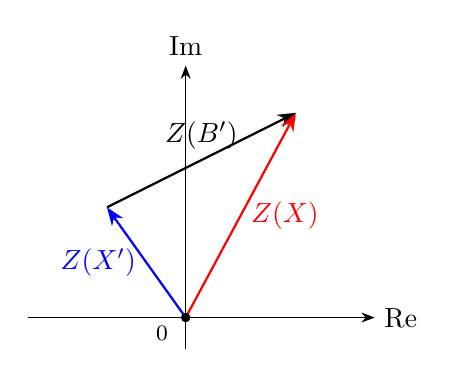
\begin{tikzpicture}[scale=2, >=Stealth]

  % 原点を中心に設定
  \coordinate (O) at (0,0);

  % 各ベクトルの終点
  \coordinate (X') at (-0.5,0.7);     % Z(A)
  \coordinate (B') at (1.2,0.6);    % Z(X/A)
  \coordinate (X) at ($(X')+(B')$); % Z(X) = Z(A) + Z(X/A)

  % 軸
  \draw[->] (-1,0) -- (1.2,0) node[right] {\(\Re\)};
  \draw[->] (0,-0.2) -- (0,1.6) node[above] {\(\Im\)};

  % Z(A) ベクトル(青)
  \draw[->, thick,blue] (O) -- (X') node[midway, left] {\(Z(X')\)};

  % Z(X/A) ベクトル(緑):Aの先から
  \draw[->, thick] (X') -- (X) node[midway,above] {\(Z(B')\)};

  % Z(X) ベクトル(赤):原点から
  \draw[->, thick,red] (O) -- (X) node[midway, right] {\(Z(X)\)};

  % 原点
  \fill (O) circle (0.03);
  \node at (-0.15, -0.1) {\footnotesize 0};

\end{tikzpicture}
\end{center}

		Step 2\\
			$X\twoheadrightarrow B$が次の条件をみたすとき極大不安定商(mdq)と呼ぶ.\\
			\bullet $\phi(X)\ge\phi(B)$\\
			\bullet 任意の$X\twoheadrightarrow B'$に対して,$\phi(B')\ge \phi(B)$であり,$\phi(B')=\phi(B)$なら
			\[X\twoheadrightarrow B\twoheadrightarrow B'.\]
			と分解.\\
			このとき,任意の対象$X$はmdqを持つことがわかる.
	$X\twoheadrightarrow B'$において$B'$が半安定でないならStep 1から半安定な対象$B''$で$\phi(B')>\phi(B'')$と$B'\twoheadrightarrow B''$がとれるので,$B'$が半安定なときについて示せばよい.同様にmdqの$B$は半安定でなければならない.\\
$X$が半安定対象のとき,任意の全射$X\twoheadrightarrow B'$に対して,短完全列
\[0\rightarrow \Ker f\rightarrow X\xrightarrow{f} B'\rightarrow 0.\]
が存在するので$Z(B') = Z(X) - Z(\Ker f)$.安定対象なので,$\phi(\Ker f)\le \phi(X)$
\begin{center}
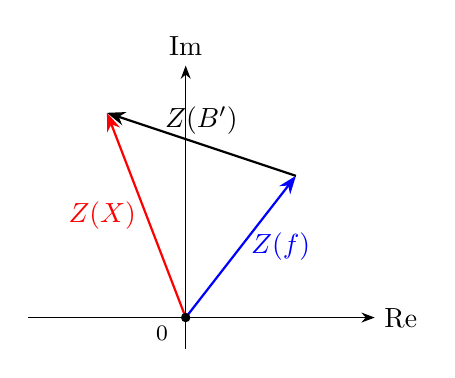
\begin{tikzpicture}[scale=2, >=Stealth]

  % 原点を中心に設定
  \coordinate (O) at (0,0);

  % 各ベクトルの終点
  \coordinate (Ker) at (0.7,0.9);     % Z(A)
  \coordinate (B') at (-1.2,0.4);    % Z(X/A)
  \coordinate (X) at ($(Ker)+(B')$); % Z(X) = Z(A) + Z(X/A)

  % 軸
  \draw[->] (-1,0) -- (1.2,0) node[right] {\(\Re\)};
  \draw[->] (0,-0.2) -- (0,1.6) node[above] {\(\Im\)};

  % Z(A) ベクトル(青)
  \draw[->, thick,blue] (O) -- (Ker) node[midway, right] {\(Z(\Ker f)\)};

  % Z(X/A) ベクトル(緑):Aの先から
  \draw[->, thick] (Ker) -- (X) node[midway,above] {\(Z(B')\)};

  % Z(X) ベクトル(赤):原点から
  \draw[->, thick,red] (O) -- (X) node[midway, left] {\(Z(X)\)};

  % 原点
  \fill (O) circle (0.03);
  \node at (-0.15, -0.1) {\footnotesize 0};

\end{tikzpicture}
\end{center}
したがって,$\phi(B')\ge\phi(X)$となり$X$が半安定対象のとき,$X\xrightarrow{\id}X$はmdqとなる.\\
そうでないとき,step1より$\phi(A)>\phi(X)$なる半安定対象$A\subsetneq X$と
\[0\rightarrow A\rightarrow X\rightarrow X'\rightarrow 0.\]
という完全列が存在する.$\phi(A)>\phi(X)>\phi(X')$となっている.$X'\twoheadrightarrow B$が$X'$のmdqとなっているとき,合成$X\twoheadrightarrow B$は$X$のmdqであることを示す.\\
\because $X\twoheadrightarrow B'$を半安定で$\phi(B')\le \phi(B)$となっているとすると
\[\phi(A)>\phi(X)>\phi(X')\ge\phi(B)\ge\phi(B').\]
$A,B'$は半安定対象であり,前の補題より$\Hom_{\D}(A,B')=0$
\[\begin{tikzcd}
	A \ar[r,hookrightarrow]\ar[rd,"0",swap,]& X\ar[r,twoheadrightarrow]\ar[d,twoheadrightarrow]& X/A = X'\ar[ld,dotted,two heads].\\
								 &B'
\end{tikzcd}\]
図式のように可換にする全射が普遍性から存在する.$X'\twoheadrightarrow B$がmdqなので$\mu(B')=\mu(B)$となり,mdqの条件より$X'\twoheadrightarrow B\twoheadrightarrow B'$と経由する.したがって$X\twoheadrightarrow B\twoheadrightarrow B'$が存在し,$X\twoheadrightarrow B$がmdqであることがわかる.\\
$X'$がmdqでない場合は$X$を$X'$に取り替えて議論を繰り返すことと条件(ii)から有限回でとまるのでmdqの存在がわかる.

		Step 3\\
		任意の$X\in\A$はHN分解をもつ.
	$0$でない$X\in\A$を任意にとる.$X$が半安定なら$0\subset X$がHN分解を与えている.そうでないとき,$X\twoheadrightarrow B^1$をmdqとして
	\[0\rightarrow X^1 \rightarrow X\rightarrow B^1\rightarrow 0.\]
	をとる.$X^1$が半安定であるなら$0\subsetneq X^1\subsetneq X$がHN分解になっている.($X/X^1\simeq B$でmdqの$B$が半安定であるため).$X^1$がmdqでないとき,$X^1\twoheadrightarrow B^2$をmdqとして
	\[0\rightarrow X^2\rightarrow X^1\rightarrow B^2\rightarrow 0.\]
	$Q=X/X^2$とすると,$X\twoheadrightarrow B^1$がmdqであることから$\phi(Q)\ge\phi(B^1)$であり,次の短完全列
	\[0\rightarrow B^2\rightarrow Q\rightarrow B^1\rightarrow 0.\]
	\begin{center}
	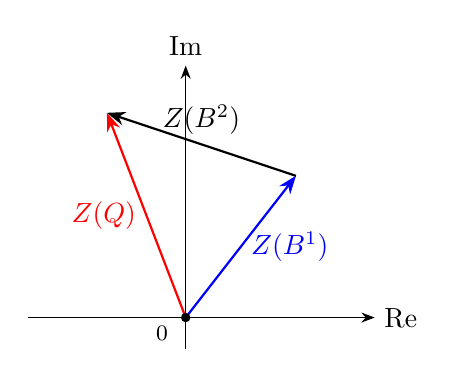
\begin{tikzpicture}[scale=2, >=Stealth]

		% 原点を中心に設定
		\coordinate (O) at (0,0);

		% 各ベクトルの終点
		\coordinate (B1) at (0.7,0.9);     % Z(A)
		\coordinate (B2) at (-1.2,0.4);    % Z(X/A)
		\coordinate (Q) at ($(B1)+(B2)$); % Z(X) = Z(A) + Z(X/A)

		% 軸
		\draw[->] (-1,0) -- (1.2,0) node[right] {\(\Re\)};
		\draw[->] (0,-0.2) -- (0,1.6) node[above] {\(\Im\)};

		\draw[->, thick,blue] (O) -- (B1) node[midway, right] {\(Z(B^1)\)};

		\draw[->, thick] (B1) -- (Q) node[midway,above] {\(Z(B^2)\)};

		\draw[->, thick,red] (O) -- (Q) node[midway, left] {\(Z(Q)\)};

		% 原点
		\fill (O) circle (0.03);
		\node at (-0.15, -0.1) {\footnotesize 0};

	\end{tikzpicture}
\end{center}
から$\phi(B^2)\ge\phi(Q)$が得られる.$\phi(B^2)=\phi(Q)=\phi(B^1)$と仮定すると,$X\twoheadrightarrow B^1$がmdqであることから$X\twoheadrightarrow B^1\twoheadrightarrow Q$となって,$B^1$と$Q$の双方向に全射があることから$B^1\simeq Q$となり,$B^2=0$.これは矛盾.したがって,$\phi(B^2)>\phi(B^1)$が成り立つ.この操作は条件(ii)より有限回でとまり,その商は半安定なのでHN分解を得る.
\end{proof}


%\begin{defn}\cite{Bri07}
%	$\D\colon$三角圏.$\D$上の安定性条件とは,$\D$の有界な$t$-構造のHeart $\A\subset\D$と$\A$と$\A$上の安定性条件
%	\[Z\colon K(\D)=K(\A)\to\CC\]
%	$(Z,\A)$のことである.
%\end{defn}

\section{Bridgeland安定性条件の空間}
\begin{defn}\cite{Bri07}
$\mathrm{Slice(\D)}$を$\D$上のスライスの集合,$\mathcal P,\mathcal Q\in\mathrm{Slice} \D$に対して,
\[d(\mathcal P,\mathcal Q)\coloneq\sup_{0\neq E\in\D}\{|\phi^-_{\P}(E)-\phi_{\Q}^-(E)|,|\phi^+_{\P}(E)-\phi_{\Q}^+(E)|\}.\]
と定義する.$(\mathrm{Slice(\D)},d)$は,距離空間である.
\end{defn}
\begin{lemm}
	$\phi_{*}^+(E),\phi_{*}^-(E)\colon \mathrm{Slice(\D)}\rightarrow\RR$
	は連続写像である.
\end{lemm}
\begin{proof}
	$d(\P,\Q)=0$とすると,$0$でない$\P(\phi)$の対象は$\Q(\phi)$の対象である.したがって,$\P=\Q$.対称性,三角不等式は,絶対値と$\sup$の定義よりしたがう.
\end{proof}

ある有限生成自由アーベル群 $\Gamma$ とGrothendieck群 $K(\D)$ からの群準同型
\[
v \colon K(\D) \to \Gamma .
\]
をひとつとり,固定する.
\begin{defn}[台条件(support property)]\cite{Bri07}
三角圏 $\D$ 上の安定性条件 $\sigma = (Z, \mathcal{P})$ が次の条件が成立するとき,台条件を満たすという:\\
$C > 0$ とノルム\ $\|\cdot\|\colon\Gamma \otimes_{\mathbb{Z}} \mathbb{R} $ が上に存在して,任意の $\sigma$-安定対象 $E \in \D$ に対して
\[
\|v(E)\| \leq C \cdot |Z(v(E))| .
\]
が成立することである.
\end{defn}

\begin{prop}\cite{Bri07}
$K(\D)$ から有限自由アーベル群 $\Gamma$ への固定された群準同型$v \colon K(\D) \to \Gamma$
に対して,$\Stab_\Gamma(\D)$ は次の集合である:
\[
\Stab_\Gamma(\D) \subset \Hom_{\ZZ}(\Gamma, \CC)\times\Slice(\D).
\]
安定性条件の組$(Z,\P)$で台条件をみたすものである.この集合は,忘却写像:
		\[
			\begin{array}{ccccc}
				\mathrm{Stab}_{\Gamma}(\D)& \longrightarrow & \Hom_{\ZZ}(\Gamma,\CC) \\
				\rotatebox{90}{\in}& &\rotatebox{90}{\in}\\
				(Z,\P) & \longmapsto &  Z& .
					\end{array}
\]
は局所同相写像である.とくに,$\Stab_{\Gamma}(\D)$に$\Hom_{\ZZ}(\Gamma,\CC)$の標準的な複素構造に関して,上記の忘却写像が正則写像になるような複素構造が一意に定まる.
\end{prop}
\begin{proof}
	この写像が局所的に単射であることを示す.$\sigma = (Z,\P),\ \tau = (Z,\Q)\in \Stab_{\Gamma}(\D)$の2点に対し,$d(\P,\Q)<1$を満たすなら$\P = \Q$となることを背理法で示す.\\
	$\P\neq \Q$と仮定する.このとき,ある$\phi\in\RR$と$E\in\P(\phi)$が存在して,$E\notin\Q(\phi)$となる.このとき,$Z(E)\in\RR_{>0}e^{i\pi\phi}$である.\\
	$E\in\Q(\ge\phi)$とすると,$d(\P,\Q)<1$より,$E\in\Q([\phi,\phi +1))$となり,$E\notin Q(\phi)$だったので,
	$Z(E)\in\RR_{>0} e^{i\pi\phi}$に矛盾.同様に$E\notin \Q(\P)$も言えることから,
	\[A\rightarrow E\rightarrow B\rightarrow A[1].\]
	で$A\in\Q((\phi,\phi+1))\backslash \{0\},B\in\Q((\phi-1,\phi))\backslash \{0\}$となるものが存在する.
	$d(\P,\Q)<1$より,$A\in\P((\phi-1,\phi +2))$となる.\\
	$A\in\P((\phi -1,\phi])$であるなら,$\sigma$と$\tau$が同じ中心電荷を持つことになり矛盾.したがって,$\psi >\phi$と$C\in\P(\psi)$と$0$ではない分解の射が存在する.
\end{proof}

\section{$\qgr R$の定義}

以下$R$を可換環とする.
\begin{defn}
$\A$ をアーベル圏,$\B \subset \A$ を Serre 部分圏とする.すなわち,$\B$ は次の条件を満たす:
\begin{itemize}
  \item 任意の短完全列
  \[
  0 \to X \to Y \to Z \to 0.
  \]
  が $\A$ にあり,$Y$ が $\B$ に属するとき,$X$ および $Z$ も $\B$ に属する(逆も同様).
\end{itemize}
このとき,$\B$ による $\A$ のSerre 商圏(Serre quotient category)$\A/\B$ は次のように定義される:
\begin{itemize}
  \item 対象は $\A$ の対象と同じである.:
		\[\Ob(\A/\B)\coloneq \Ob(\A).\]
  \item 射は以下のように定義される:
  \[
  \Hom_{\A/\B}(X, Y) := \varinjlim_{\substack{X' \subset X\\ X/X' \in \B}} \varinjlim_{\substack{Y' \subset Y\\ Y' \in \B}} \Hom_{\A}(X', Y/Y').
  \]
\end{itemize}
\end{defn}

\begin{defn}[次数付き環]
環 $R$ が,アーベル群としての直和
\[ R = \bigoplus_{i \in \mathbb{Z}} R_i. \]
に分解され,かつ,環の積が任意の $i, j \in \mathbb{Z}$ に対して
\[ R_i R_j \subseteq R_{i+j} .\]
をみたすとき,$R$ を次数付き環 (graded ring) という.
このとき,$R_i$ の元を次数 $i$ の斉次元 (homogeneous element of degree $i$) と呼ぶ.
\end{defn}
以降,特に断りのない限り,次数付き環はネーター環であり,$R_0$ 上有限生成であるものとする.

\begin{defn}[次数付き加群]
$R = \bigoplus_{i \in \mathbb{Z}} R_i$ を次数付き環とし,$M$ を右 $R$-加群とする.
$M$ が部分加群の直和
\[ M = \bigoplus_{n \in \mathbb{Z}} M_n. \]
と表され、かつ、任意の $i, j \in \mathbb{Z}$ に対して、環の作用が
\[ R_i M_j \subseteq M_{i+j} .\]
をみたすとき、$M$ を次数付き$R$-加群 (graded $R$-module) という。
このとき、$M_n$ の元を次数 $n$ の斉次元 (homogeneous element of degree $n$) と呼ぶ。
\end{defn}
	
\begin{defn}
	 \( R = \bigoplus_{n \ge 0} R_n \)を次数付き環,\( M \in \gr R \)を$R$上の次数付き加群とする. $M$の元\( x \in M \) に対して,ある整数 \( n \gg 0 \) が存在して,\( R_{\ge n} \cdot x = 0 \) となるとき, 捻れ元(torsion element) であるという.ここで \( R_{\ge n} = \bigoplus_{m \ge n} R_m \) とする.

すべての元 \( x \in M \) が捻れ元である加群 \( M \)のことを捻れ加群(torsion module) であるという.このような加群全体のなす充満部分圏を \(\tors R\) で表す.
\end{defn}

\begin{prop}
次数付き環 \( R = \bigoplus_{n \ge 0} R_n \) に対し,その上の次数付き右$R$-加群全体のアーベル圏 \(\gr R\) において,torsion 加群全体からなる部分圏 \(\tors R\) は Serre部分圏である.
\end{prop}

\begin{defn}\cite{AZ94}
\(
R = \bigoplus_{n \ge 0} R_n
\) を次数付きネーター$\CC$-代数とする.\vspace{-3mm}
\begin{itemize}
  \item $\gr R$ は $\mathbb{Z}$-次数付き有限生成$R$-加群のアーベル圏とする.
  \item $\tors R$ は $\gr R$ のうち,ねじれ加群全体とする.
  \item $\qgr R$ は $\gr R$ の Serre 部分圏 $\tors R$ による商圏:$\qgr R := \gr R / \tors R$ と定義する.
\end{itemize}
\end{defn}

\begin{defn}\cite{GL87}
重み付き射影直線(weighted projective line)とは,以下のデータによって定まる射影曲線である:

\begin{itemize}
  \item 正の整数からなる列 $A = (a_0, a_1, \dots, a_r)$,
  \item $\mathbb{P}^1(k)$ の互いに異なる点の列 $\Lambda = (\lambda_0, \lambda_1, \dots, \lambda_r)$,
\end{itemize}

ただし,通常 $\lambda_0 = \infty,\ \lambda_1 = 0,\ \lambda_2 = 1$ と正規化する.次に,アーベル群
\[
	L_{A} \coloneq \ZZ \vec{x_1}\oplus\cdots\oplus\ZZ \vec{x_r}\oplus \ZZ\vec{c}\Big{/}\langle\vec{c} -a_i\vec{x_i}\mid i=1,\ldots,r\rangle.
\]
を定義し,これを次数付き群とする.多項式環: 
\[
	S = k[X_0, X_1, \dots, X_r], \quad \deg X_i = \vec{x}_i. 
\]
において,以下の $L_A$-斉次イデアル:
\[
	I_{A,\Lambda} = \left( X_i^{a_i} - X_1^{a_1} + \lambda_i X_0^{a_0} \ \middle|\ i = 2, \dots, r \right).
\]
を用いて商環
\[
	R_{A,\Lambda} = k[X_0, X_1, \dots, X_r]\Big{/}I_{A,\Lambda} = k[x_0,x_1,\ldots, x_r],\quad \deg(x_i)=\vec{x_i}.
\]
を定義する.このとき,$R_{A,\Lambda}$は,部分環$k[x_0^{a_0},x_1^{a_1}]$が存在する.
\end{defn}

$L_A$は階数$1$のアーベル群であり,各次数$\vec{\ell}\in L_A$は一意的に,
\[\vec{\ell} = \sum_{i=0}^r \ell_i\vec{x_i} + \ell\vec{c}\quad (0\le \ell_i < p_i,\ \ \ell \in \ZZ).\]
と表すことができる.
ここで,
\[\vec{\omega} \coloneq (r-1)\vec{c} - \sum_{i=0}^r\vec{x_i}.\]
と$\vec{\omega}$を定義し,双対化元(dualizing element)と呼ぶ.また,
\[R(A)= \bigoplus_{\ell=0}^\infty R_{\ell},\quad R_\ell = S_{\ell\vec{c}}.\]
を$R_{A,\Lambda}$の核(core)と呼ぶ.

\begin{defn}\cite{GL87}
	Serreの定理より,重み付き射影直線 $\mathbb{X}$に対応する $L_A$-次数付き環 $R_{A,\Lambda}$ に対して,次のように連接層の圏$\Coh(\mathbb{X})$ を定義する:

\[
\Coh(\mathbb{X}) := \qgr R_{A,\Lambda} = \gr R_{A,\Lambda}\Big{/}\tors R_{A,\Lambda}.
\]

ここで,
\begin{itemize}
	\item $\gr R_{A,\Lambda}$ は $L_A$-次数付き有限生成$R_{A,\Lambda}$-加群の圏,
	\item $\tors R_{A,\Lambda}$ は $\gr R_{A,\Lambda}$のねじれ加群全体の圏.
\end{itemize}
このとき,2つの圏の間には自然な射影函手 (projection functor)を
\[ \pi: \gr R_{A,\Lambda} \longrightarrow \Coh(\XX) .\]
と記す.さらに,$\vec{x} \in L(\mathbf{p})$ に対して,ひねり(twist)とは,$R_{A,\Lambda}$-加群 $M$ に対して次のように定義される加群 $M(\vec{x})$ を与える操作である:
\[
M(\vec{x})_{\vec{y}} := M_{\vec{x} + \vec{y}} \quad (\vec{y} \in L(\mathbf{p})).
\]
$(M,\vec{x})\to M(\vec{x})$により,各圏に対して$L_A$作用が定まる.
\end{defn}
$R_{A,\Lambda}(\vec{x})$ を射影函手 $\pi$ で写した $\mathrm{coh}(\mathcal{X})$ の対象を,
\[ \mathcal{O}(\vec{x}) := \pi(R(\vec{x})). \]
と書き,(次数 $\vec{x}$ による)捩り層 (twisting sheaf) と呼ぶ.\\

$x = $
\[0\longrightarrow \mathcal{O}\xrightarrow{\ u\ }\mathcal{O}(\vec{c})\longrightarrow S\longrightarrow 0\]
$L_{A,\Lambda}$ の元 $\vec{x}, \vec{y}$ に対する順序を以下のように定義する.
\begin{center}
  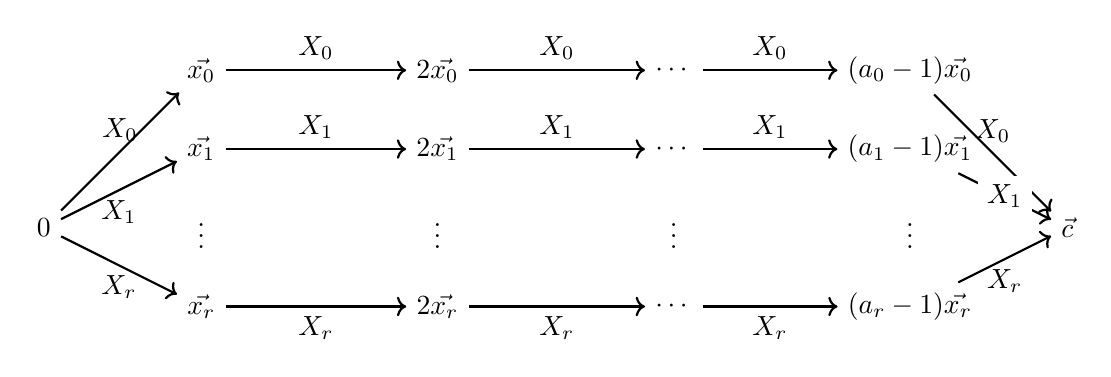
\begin{tikzpicture}[->,thick]
      \node (0) at (0,0) {0};
			\node (11) at (2,2) {$\vec{x_0}$};
			\node (12) at (5,2) {$2\vec{x_0}$};
      \node (13) at (8,2) {$\cdots$};
			\node (14) at (11,2) {$(a_0-1)\vec{x_0}$};
      \node (21) at (2,1) {$\vec{x_1}$};
      \node (22) at (5,1) {$2\vec{x_1}$};
      \node (23) at (8,1) {$\cdots$};
			\node (24) at (11,1) {$(a_1-1)\vec{x_1}$};
      \node (31) at (2,0) {$\vdots$};
      \node (32) at (5,0) {$\vdots$};
      \node (33) at (8,0) {$\vdots$};
      \node (34) at (11,0) {$\vdots$};
			\node (41) at (2,-1) {$\vec{x_r}$};
			\node (42) at (5,-1) {$2\vec{x_r}$};
      \node (43) at (8,-1) {$\cdots$};
			\node (44) at (11,-1) {$(a_r-1)\vec{x_r}$};
			\node (1) at (13,0) {$\vec{c}$};
      \draw (0) -- node[above] {$X_0$} (11);
      \draw (11) -- node[above] {$X_0$} (12);
      \draw (12) -- node[above] {$X_0$} (13);
      \draw (13) -- node[above] {$X_0$} (14);
      \draw (14) -- node[above] {$X_0$} (1);
      \draw (0) -- node[below] {$X_1$} (21);
      \draw (21) -- node[above] {$X_1$} (22);
      \draw (22) -- node[above] {$X_1$} (23);
      \draw (23) -- node[above] {$X_1$} (24);
      \draw (24) -- node[pos=.5,fill=white] {$X_1$} (1);
      \draw (0) -- node[below] {$X_r$} (41);
      \draw (41) -- node[below] {$X_r$} (42);
      \draw (42) -- node[below] {$X_r$} (43);
      \draw (43) -- node[below] {$X_r$} (44);
      \draw (44) -- node[below] {$X_r$} (1);
  \end{tikzpicture}
  \end{center}

\begin{thm}[Krull--Schmidt 性]\cite{GL87}
重み付き射影直線 $\mathbb{X} $ に対して,連接層のアーベル圏
\[
\Coh(\mathbb{X}) = \qgr R_{A,\Lambda} = \gr R_{A,\Lambda}\Big{/}\tors R_{A,\Lambda}.
\]
は Krull--Schmidt 圏である.すなわち,任意の対象 $\mathcal{F} \in \Coh(\mathbb{X})$ は直既約対象の有限直和に分解でき,その分解は同型と順序を除いて一意である:
\[
\mathcal{F} \cong \bigoplus_{i=1}^n \mathcal{F}_i \quad (\text{各} \mathcal{F}_i \text{が既約対象}).
\]
\end{thm}

\begin{lemm}
	重み付き射影直線 $\mathbb{X}$において,各直線束$L$は$\Coh(\XX)$における例外対象である.
\end{lemm}
\begin{proof}
	$L = \mathcal{O}(\vec{x})$とかけるので,
	\[\Hom(\mathcal{O}(\vec{x}),\mathcal{O}(\vec{x}))=S_0=k.\]
	である.
\end{proof}

\begin{thm}\cite{GL87}
重み付き射影直線 $\mathbb{X}$ において,次の加群
\[
T := \bigoplus_{0 \le \vec{x} \le \vec{c}} \mathcal{O}_{\mathbb{X}}(\vec{x}).
\]
をとると,これは $\Coh(\mathbb{X})$ における傾対象である.
\end{thm}

\begin{thm}[Serre 双対性]\cite{GL87}
重み付き射影直線 $\mathbb{X}$ において,任意の連接層 $\mathcal{F}, \mathcal{G} \in \Coh(\mathbb{X})$ に対して,次の自然なベクトル空間の同型が成り立つ:
\[
\Ext^1(\mathcal{F}, \mathcal{G})^\vee \cong \Hom(\mathcal{G}, \mathcal{F}(\vec{\omega})).
\]
\[
\RHom(\F,\G)^\vee \simeq \RHom(\G,\F(\vec{\omega}))[1]?\]
ここで,
\begin{itemize}
	\item $(-)^\vee := \Hom_{\CC}(-, \CC)$ は $\CC$ 上の線型双対,
  \item $\vec{\omega} = (n - 1)\vec{c} - \sum_{i=0}^n \vec{x}_i$ は dualizing element(双対化元)である.
\end{itemize}
この同型は $\mathcal{F}, \mathcal{G}$ に関して函手的である.
\end{thm}

\begin{exmp}
$R = \CC[x, y]$ を $\ZZ$次数付き多項式環とし,$\deg(x) = 1$,$\deg(y) = 2$ とする.このとき,$R$ は重み付き射影直線 $\mathbb{P}(1,2)$ に対応し,次のような圏同値が成り立つ:
\[
\qgr R := \gr R / \tors R \simeq \Coh(\mathbb{P}(1,2)).
\]
\[
R := \CC[x, y], \quad \deg(x) = 1,\quad \deg(y) = 2.
\]

各\(n \in \ZZ_{\ge 0}\) に対して次数成分 \(R_n\) は次のように与えられる:
\[
\begin{aligned}
R_0 &= \CC \\
R_1 &= \CC x \\
R_2 &= \CC x^2 \oplus \CC y \\
R_3 &= \CC x^3 \oplus \CC x y \\
R_4 &= \CC x^4 \oplus \CC x^2 y \oplus \CC y^2 \\
&\vdots 
\end{aligned}
\]

このとき,次の列
\[
(\mathcal{O},\ \mathcal{O}(1),\ \mathcal{O}(2)),
\]
は \(\D^b(\Coh(\mathbb{P}(1,2)))\) における強例外生成列(\ref{defn:strong exceptional collection})であり,その直和
\[
T := \mathcal{O} \oplus \mathcal{O}(1) \oplus \mathcal{O}(2),
\]
は傾斜対象(\ref{defn:tilting object})となる.したがって,導来函手
\[
\RHom(T, -) \colon \D^b(\Coh(\mathbb{P}(1,2))) \longrightarrow \D^b(\mod \End(T)).
\]
は三角同値を与える.
\end{exmp}


\section{GL}
\begin{defn}\cite{GL87}
重み付き射影直線(weighted projective line)とは,以下のデータによって定まる射影曲線である:

\begin{itemize}
  \item 正の整数からなる列 $\mathbf{p} = (p_0, p_1, \dots, p_n)$,
  \item $\mathbb{P}^1(k)$ の互いに異なる点の列 $\boldsymbol{\lambda} = (\lambda_0, \lambda_1, \dots, \lambda_n)$,
\end{itemize}

ただし,通常 $\lambda_0 = \infty,\ \lambda_1 = 0,\ \lambda_2 = 1$ と正規化する.次に,アーベル群
\[
L(\mathbf{p}) = \left\langle \vec{x}_0, \vec{x}_1, \dots, \vec{x}_n \ \middle| \ p_0 \vec{x}_0 = p_1 \vec{x}_1 = \cdots = p_n \vec{x}_n \right\rangle .
\]
を定義し,これを次数付き群とする. $\vec{c}\coloneq p_0 \vec{x}_0 = \cdots = p_n \vec{x}_n$ と定める.

$L(\mathbf{p})$ によって次数付けされた多項式環:
\[
S = \CC[X_0, X_1, \dots, X_n], \quad \deg X_i = \vec{x}_i.
\]
において,以下の $L(\mathbf{p})$-斉次イデアル:
\[
I(\mathbf{p}, \boldsymbol{\lambda}) = \left( X_i^{p_i} - X_1^{p_1} + \lambda_i X_0^{p_0} \ \middle|\ i = 2, \dots, n \right).
\]
を用いて商環
\[
S(\mathbf{p}, \boldsymbol{\lambda}) = \frac{k[X_0, X_1, \dots, X_n]}{I(\mathbf{p}, \boldsymbol{\lambda})}.
\]
を定義する.この $L(\mathbf{p})$-次数付き環 $S(\mathbf{p}, \boldsymbol{\lambda})$ を用いて,次のように構成される代数多様体
\[
\mathbb{X} = \mathbb{C}(\mathbf{p}, \boldsymbol{\lambda}) = \mathrm{Proj}_{L(\mathbf{p})}(S(\mathbf{p}, \boldsymbol{\lambda})).
\]
を重み付き射影直線(weighted projective line)と呼ぶ.
\end{defn}
ここで,
\[\vec{\omega} \coloneq (n-1)\vec{c} - \sum_{i=0}^n\vec{x_i}.\]
と$\vec{\omega}$を定義し,双対化元(dualizing element)と呼ぶ.

\begin{defn}\cite{GL87}
重み付き射影直線 $\mathbb{X} = \mathbb{C}(\mathbf{p}, \boldsymbol{\lambda})$ に対応する $L(\mathbf{p})$-次数付き環 $S = S(\mathbf{p}, \boldsymbol{\lambda})$ に対して,次のように連接層の圏$\Coh(\mathbb{X})$ を定義する:

\[
\Coh(\mathbb{X}) := \frac{\mathrm{mod}^{L(\mathbf{p})}_+(S)}{\mathrm{mod}^{L(\mathbf{p})}_0(S)}.
\]

ここで,
\begin{itemize}
  \item $\mathrm{mod}^{L(\mathbf{p})}_+(S)$ は $L(\mathbf{p})$-次数付き有限生成 $S$-加群の圏,
  \item $\mathrm{mod}^{L(\mathbf{p})}_0(S)$ は $L(\mathbf{p})$-次数付き有限長 $S$-加群(すなわち有限サポートをもつ加群)の圏.
\end{itemize}
\end{defn}

\begin{thm}[Serre 双対性]\cite{GL87}
重み付き射影直線 $\mathbb{X} = \mathbb{C}(\mathbf{p}, \boldsymbol{\lambda})$ において,任意の連接層 $\mathcal{F}, \mathcal{G} \in \Coh(\mathbb{X})$ に対して,次の自然なベクトル空間の同型が成り立つ:
\[
\Ext^1(\mathcal{F}, \mathcal{G})^\vee \cong \Hom(\mathcal{G}, \mathcal{F}(\vec{\omega})).
\]
\[
\RHom(\F,\G)^\vee \simeq \RHom(\G,\F(\vec{\omega}))[1]?\]
ここで,
\begin{itemize}
	\item $(-)^\vee := \Hom_{\CC}(-, \CC)$ は $\CC$ 上の線型双対,
  \item $\vec{\omega} = (n - 1)\vec{c} - \sum_{i=0}^n \vec{x}_i$ は dualizing element(双対化元)である.
\end{itemize}
この同型は $\mathcal{F}, \mathcal{G}$ に関して函手的である.
\end{thm}


\section{行列因子化の圏}
\begin{defn}\cite{KST06}
	多項式$f$に対して,次数付き行列因子化$M$を次のように定義する:
\[M\coloneq\mf{P_0}{p_0}{p_1}{P_1},\]
$P_0,P_1$は次数付き有限階数自由右$R$-加群,$p_0\colon P_0\rightarrow P_1$は次数$0$の$R$-準同型,$p_1\colon P_1\rightarrow P_0$は次数$2$の$R$-準同型であって,$p_1p_0 = f\cdot\id_{P_0},\ p_0p_1 = f\cdot\id_{P_1}$となるものである.$f$のすべての次数付き行列因子化の集合を$\mathrm{MF}^{\text{gr}}_{R}(f)$と記す.\\
2つの次数付き行列因子化$\ M= \mf{P_0}{p_0}{p_1}{P_1},\ M' =\mf{P_0'}{p_0'}{p_1'}{P_1'}\in\mathrm{MF}^{\text{gr}}_{R}(f)$に対して,その間の射$\Phi = (\phi_0,\phi_1)$を以下のように定める:\\
次数0の$R$-準同型:$\phi_0\colon P_0 \rightarrow P_0'\ \phi_1\colon P_1 \rightarrow P_1' $であって,以下の図式を可換にするもの:
		\[
		\begin{tikzcd}
			P_0\ar[r,"p_0"]\ar[d,"\phi_0"]& P_1\ar[r,"p_1"]\ar[d,"\phi_1"]& P_0\ar[d,"\phi_0"]\\
			P_0'\ar[r,"p_0'",swap]& P_1'\ar[r,"p_1'",swap]& P_0' .
		\end{tikzcd}
	\]
\end{defn}

\begin{defn}\cite{KST06}
	次数付き行列因子化の加法圏$\mathrm{HMF}^{\text{gr}}_{R}(f)$を以下のように定める:
	\[\Ob(\mathrm{HMF}^{\text{gr}}_{R}(f)) \coloneq \mathrm{MF}^{\text{gr}}_{R}(f).\]
	任意の$M,M'\in \mathrm{MF}^{\text{gr}}_{R}(f)$に対して,
	\[\Hom_{\mathrm{HMF}^{\text{gr}}_{R}(f)}(M,M')\coloneq \Hom_{\mathrm{MF}^{\text{gr}}_{R}(f)}(M,M')/\mathbin{\sim}.\]
	ここで,$\Phi,\Phi'\in\Hom_{\mathrm{MF}^{\text{gr}}_{R}(f)}(M,M')$に対して,次数0の$R$-準同型の組:$(h_0,h_1)\colon (P_0\to P_1), (P_1\to P_0)$であって,$\Phi- \Phi' = (\tau^{-h}(p_1')h_0 + h_1p_0,\ p_0'h_1 + \tau^h(h_0)p_1)$となるようなものが存在するとき,同値$\Phi\sim\Phi'$と定める.
		\[
		\begin{tikzcd}
			P_0\ar[r,"p_0"]\ar[d,"\phi_0",swap]& P_1\ar[r,"p_1"]\ar[d,"\phi_1",swap]\ar[ld,"h_1"description,dotted]& P_0\ar[d,"\phi_0"]\ar[ld,"h_0"description,dotted]\\
			P_0'\ar[r,"p_0'",swap]& P_1'\ar[r,"p_1'",swap]& P_0' .
		\end{tikzcd}
	\]
	ただし,$\tau = (1)$は次数シフトである.
\end{defn}

$M= \mf{P_0}{p_0}{p_1}{P_1}\in\mathrm{HMF}^{\text{gr}}_{R}(f)$に対し,
\[P_0 = b_1R\oplus\cdots\oplus b_rR,\quad P_1 = \overline{b_1}R\oplus\cdots \overline{b_r}R.\]
となるような,基底$b_1,\ldots, b_r,\overline{b_1},\ldots, \overline{b_r}$をとると,$2r\times 2r$の行列の組$(Q,S)$で表すことができる.ここで,
\begin{gather*} Q = \begin{pmatrix}
	0 & \phi\\
	\psi & 0
\end{pmatrix},\quad \varphi,\psi \in \Mat_r(R),\\
S = \begin{pmatrix}
	s_1\\
	&\ddots\\
	& & s_r\\
	& & &\overline{s_1}\\
	& & & &\ddots\\
	& & & &&\overline{s_1}\\
\end{pmatrix},\quad s_i = \deg(b_i),\ \overline{s_i} = \deg(\overline{b_i}) - 1.
\end{gather*}
であり,
\[Q^2 = f\cdot I_{2r},\quad -SQ + QS + 2EQ = Q. {\color{red}{why?}}\]

\begin{thm}\cite{KST06}
	$f\in\CC[x,y,z]$をADE型の多項式とし,$\vec{\Delta}$を対応する向きが固定されたディンキン箙とする.このとき,以下の三角圏の同値が存在する:
	\[\mathrm{HMF}^{\text{gr}}_{R}(f)\simeq D^b(\mod \CC\vec{\Delta}).\]
\end{thm}

\begin{defn}\cite{KST06}
	次数付き行列因子化$M = (Q,S)\in\mathrm{HMF}^{\text{gr}}_{R}(f) $に対して,複素数を以下のように対応させる:
	\[\Z(M) \coloneq \Tr(e^{\pi\sqrt{-1}S}).\]
	これをグロタンディーク群上に線型に延長する$\Z\colon K(\mathrm{HMF}^{\text{gr}}_{R}(f))\to\CC$.
\end{defn}

\begin{thm}\cite{KST06}
	$f\in R$をADE型の多項式とする.$\P(\phi)$を$\mathrm{HMF}^{\text{gr}}_{R}(f)$の位相$\phi$の既約対象から生成される充満部分加法圏とする.このとき,$(P(\phi),\Z)$は,$\mathrm{HMF}^{\text{gr}}_{R}(f)$上にBridgeland安定性条件をさだめる.
\end{thm}


\begin{thebibliography}{99}

	\bibitem[Tod13]{Tod13}
	Yukinobu Toda
		\textit{Gepner type stability conditions on graded matrix factorizations},

	\bibitem[MMS09]{MMS09}
Emanuele Macri, Sukhendu Mehrotra, Paolo Stellari
		\textit{Inducing stability conditions},
	
	\bibitem[KS08]{KS08}
	Maxim Kontsevich, Yan Soibelman
		\textit{Stability structures, motivic Donaldson-Thomas invariants and cluster transformations},

	\bibitem[Bri07]{Bri07}
	Bridgeland, Tom,
		\textit{Stability conditions on triangulated categories},
	Annals of Mathematics, Vol. 166, No. 2, 2007, pp. 317–345.


	\bibitem[KST06]{KST06}
	Hiroshige Kajiura, Kyoji Saito, Atsushi Takahashi
		\textit{Matrix Factorizations and Representations of Quivers II: type ADE case},

	\bibitem[Tak05]{Tak05}
	 Atsushi Takahashi
		\textit{Matrix Factorizations and Representations of Quivers I},

	\bibitem[KS06]{KS06}
	Masaki Kashiwara and Pierre Schapira,
		\textit{Categories and Sheaves},
	Grundlehren der Mathematischen Wissenschaften, vol. 332,
	Springer-Verlag, Berlin, 2006.

	\bibitem[Kuz03]{Kuz03}
	\textit{Derived categories of cubic and V14 threefolds},

	\bibitem[GM03]{GM03}
	S. I. Gelfand and Yu. I. Manin,
	\textit{Methods of Homological Algebra}, 2nd ed.,
	Springer Monographs in Mathematics, Springer, 2003.

	\bibitem[AZ94]{AZ94}
	Michael Artin and James J. Zhang,
	\textit{Noncommutative Projective Schemes},
	Adv. Math. \textbf{109} (1994), no.~2, 228--287.

	\bibitem[BK89]{BK89}
	A.~Bondal and M.~Kapranov,
	\newblock Representable functors, Serre functors, and reconstructions,
	\newblock {\em Izv. Akad. Nauk SSSR Ser. Mat.} \textbf{53} (1989), no.~6, 1183--1205.
	\newblock English transl.: {\em Math. USSR Izv.} \textbf{35} (1990), no.~3, 519--541.

	\bibitem[Ri89]{Ri89}
	J.~Rickard,
	\newblock Morita theory for derived categories,
	\newblock {\em J. London Math. Soc. (2)} \textbf{39} (1989), no.~3, 436--456.


	\bibitem[GL87]{GL87}
	W.~Geigle and H.~Lenzing,
	\newblock A class of weighted projective curves arising in representation theory of finite-dimensional algebras,
	\newblock in *Singularities, Representation of Algebras, and Vector Bundles* (Lambrecht, 1985), Lecture Notes in Math. 1273, Springer, Berlin, 1987, pp. 265–297.
	
	\bibitem[BBD]{BBD}
	A. A. Beilinson, J. Bernstein, and P. Deligne,
	\textit{Faisceaux pervers},
	Astérisque, \textbf{100}, Société Mathématique de France, 1982. Chapitre 1.

	\bibitem[Gro57]{Gro57}
	A.~Grothendieck,
	\textit{Sur quelques points d'algèbre homologique},
	Tohoku Math. J. (2) \textbf{9} (1957), 119--221.

	\bibitem[Serre55]{Serre55}
	J.-P.~Serre,
	\newblock Faisceaux algébriques cohérents,
	\newblock \emph{Ann. of Math.} \textbf{61} (1955), 197--278.

\end{thebibliography}
\end{document}
